\chapter{Model Personalisation}
\label{chp:personalisation}
The previous chapter investigated classification accuracy for a general or subject agnostic \acrshort{lstm} based \acrshort{lmr} model. Due to the variability between individuals classification accuracies of greater than 80\% could not be achieved for unseen novel subjects. Instead a form of personalisation is necessary to adapt the model for novel subjects. Within this chapter methods for achieving this will be explored. Before attempting to produce a model for amputees methods will be developed and tested on non-amputees.

The collection of labelled data for an individual is burdensome therefore any system that can be used to reduce the labelling requirements is advantageous. Transfer learning approaches allow large training sets pooled from many individuals to be leveraged to reduce target data requirements on the assumption they hold relevant information.\cite{Fallahzadeh2017, Schneider2021}

From this point forward the following naming convention will be used; the subject of personalisation will be referred to as the target with all other subjects referred to as source.

Within this chapter we will investigate whether a large population of source data can be used to improve the performance and efficiency of producing a personalised \acrshort{lstm} \acrshort{lmr} classifier for a target individual.

The contributions of this Chapter are as follows:
\begin{itemize}
    \item A method for evaluating personalisation \acrshort{lmr} models from a set of real world continuous gait data
    \item Demonstration of the impact on classification performance of increased target training data
\end{itemize}

The Chapter is presented as follows. First, in Section \ref{sec:personalisation-related-works}, related literature is presented. This is followed by the methods and materials used in the study in Section \ref{sec:personalistaion-methods}. The results of a baseline model trained from only target data are presented in Section \ref{sec:personalisation-baseline-model-results}, followed by the results and analysis for personalisation techniques in Sections \ref{sec:model-personalisation-results-supplementation} and \ref{sec:model-personalisation-results-transfer}. Finally discussion and conclusions are presented in Sections \ref{sec:personalisation-discussion} and \ref{sec:personalisation-conclusions} respectively.

%------------------------------------------
\section{Related Works} % Does this need more detail to back up the research gaps identified
\label{sec:personalisation-related-works}
\acrshort{ml} classifiers are constructed with the assumption that the probabilistic distribution between the source and target domain are equal\cite{Farahani2020}. In reality this is never the case and as such methods to account for differences between domains have been developed. Where this is adaptation between humans this is typically termed personalisation.

Personalising of \acrshort{ml} models is a common issue and has been addressed in many different ways across different areas of research\cite{Mairittha2021, Tomanek2021}. Schneider et al divides personalisation methods into two groups, shaping and data grouping\cite{Schneider2021}. In shaping the behaviour of a network is biased or shaped towards an individual, in data grouping the target data set is enlarged by adding data from similar individuals to it. Both of these techniques take advantage of data from others to reduce labelled data requirements for the target subject\cite{Shor2020}. The following survey of literature will be divided by these two categories. 

Shaping the behaviour of a network can occur at different times during training. Two are common, the beginning, early, or the end, late. In early shaping the model is first trained with target data followed by a larger set of source data. The opposite is done in late shaping, where a general model formed from a large source training set is fine-tuned with target data. By updating a trained model using data from a different distribution, the knowledge from an existing model can be transferred. This method is common and normally referred to as transfer learning.\cite{Schneider2021}

Transfer learning is the ability to extend what has been learnt in one context to another nonidentical but similar context\cite{Fallahzadeh2017}. The change in context can be either the task, the domain or both. Transfer learning is appealing, since it is often faster, as a model does not need to be trained from scratch for each target. 

Transfer learning is generally achieved in two phases. First a generic global model is trained from a set of source data. Then it is adapted to the target by additional training using only the targets data. The influence of the target is controllable by both the number of iterations and number of layers trained.\cite{Schneider2021, Mireshghallah2021}

A subset of transfer learning is domain adaptation where the domain changes but the task remains the same\cite{Goodfellow2015}. Domain adaptation techniques often focus on learning and apply a mapping between the source and target input data rather than fine-tuning an existing model.

%-----------------------------
% Shaping/Transfer learning
Yoon et al presented a transfer learning scheme for personalisation of a \acrshort{lstm} based language model for generating stylised sentence completion. Their work focuses on techniques that allow transfer learning using only a small amount of target data and limited computing resource. To achieve this two schemes are investigated - inserting and training a surplus layer between the output and last LSTM layer; and freezing the first n-layer and fine-tuning just the subsequent layers. Both methods reduce the training requirements when compared to fine-tuning the entire base model while achieving similar performance.\cite{Yoon2017}

Fu et al developed a domain adaptation method for unlabelled target data denoted Joint Probability Domain Adaptation with Improved Pseudo Labels (IPL-JPDA). The method produces a transformation matrix to adapt the input data of the target to the source domain removing the need to adjust the model itself. The study collects labelled data for a set of ten subjects in a controlled environment. This data is then split into target and source data sets with the performance tested using a cross validation method. Personalisation is undertaken using the IPL-JPDA method and tested against a subset of the data windows for each activity. Their method achieves an accuracy of $93.2\%$ accuracy, an increase of around $2\%$ over the baseline.\cite{Fu2021}


%-----------------------------
% Data grouping - Training from similar users
The other category of personalisation is data grouping. In data grouping the target data set is enlarged by supplementing it with data from existing source data. Each individual will differ from each other, but it should be expected that the population as a whole or a subset of it are similar\cite{Schneider2021, Nguyen2021}. Identifying and combining similar individuals is the main area of concentration for this field.

Ferrari et al investigated data grouping personalisation methods that weight the influence of training data based on similarity to the target subject. Similarity was evaluated through physical traits (age, weight and height) and on comparison of the input feature vector. Three publicly available \acrshort{adl} data sets were used to test performance, niMiB-SHAR\cite{Micucci2017}, Mobiact\cite{Vavoulas2016} and Motion Sense\cite{Katevas2014}. All data was collected in controlled conditions. An Adaboost classifier was trained for each target subject using the weighted training data. The experiment was repeated with and without target data included in the training set. Excluding the target saw only a small improvement in performance, compared to without similarity biasing. Including the target in the training data increased classification accuracy by $>10\%$, on average achieving $87.39\%$. This suggests weighting the training data set towards the target subject has a larger influence on performance than similarity.\cite{Ferrari2020}

Nguyen et al presented another data grouping technique using a DeepConvLSTM architecture. The model used learnt features, so determining the similarity of the feature vector was not possible. Instead the output of the last LSTM layer was used as a pseudo for the feature vector. A \acrfull{fid} algorithm was used to score the similarity of subjects. The score was then used to group source subjects, by selecting the closest $n$ neighbours and also clustering subjects into communities. It was noted this correlated closely with the physical characteristics. The groups were then used to both train a new model from scratch and fine-tune a general model. Fine-tuning a global model proved more effective. This method improved the global model performance by $3.5\%$ to $84.2\%$. The experiments were performed on four public data sets; OPPORTUNITY\cite{Roggen2009}, Daphnet Gait\cite{Sigcha2020}, Wetlab\cite{Scholl2015} and Mobiact\cite{Vavoulas2016} data sets, all of which were collected in closed controlled environments.\cite{Nguyen2021}


%-----------------------------
% Combination - retrain general model based on similar users
Several authors attempted to combine both transfer learning and data grouping techniques. These methods used data grouping techniques to produce a base model which was subsequently fine-tuned using data from the target.

Wang et al presents a source selection and transfer learning approach for a \acrshort{cnn}-\acrshort{lstm} architecture for unsupervised transfer learning. First source subjects were selected based on a closeness score. This score was a combination of a cosine similarity function and a hand selected value based on physical similarity between sensor locations. Using the selected source subjects a \acrshort{ml} model was trained. Fine-tuning of the model was achieved by inserting and training an adaption layer between the last two dense layers. The investigation was performed using the OPPORTUNITY\cite{Roggen2009}, PAMAP2\cite{Reiss2012} and UCI DSADS\cite{Altun2010} data sets which again were all collected in controlled conditions.\cite{Wang2018a}

Cruciani et al presents work on personalising an activity recognition model built from the subset of a general population. The subset of subjects was selected by comparing the similarity of manually selected features. Those with the closest matching traits were used to generate the base model. Further training was then performed using a small amount of target  data. This approach achieved a ~5\% improvement in performance when compared to selecting a source subset at random\cite{Cruciani2020}. The experiment was performed on the \acrshort{adl} Extrasensory data set published by Vaizman et al\cite{Vaizman2017}, this data set was collected using a smartphone in uncontrolled conditions with limited guidance given on how to collect or label the data.

From the literature surveyed the following gaps were identified:
\begin{itemize}
\item No methods for effectively testing the general performance of a transfer learning system from continuous real world environments
\item No comparison between the performance that could be achieved by just training a model with the target subject's data
\item There has been limited work on understanding how performance improves with increasing amounts of target data
\item None have investigated the use of IMU ankle data
\end{itemize}

\hl{Add in paragraph that ties these gaps to what we are going to work on. This probably involves adjusting the gaps to match the chapter contributions.}

%------------------------------------------
\section{Methods and Materials}
\label{sec:personalistaion-methods}
%Introduction to section
Within this section, the methods and materials required to address the research question will be detailed. The section is structured as follows: first, details of an expanded data set of labelled real world HAR data are provided; then, new methods for dividing this data into representative data sets are developed; finally, \acrshort{ml} personalisation methods are presented.

% Data collection
\subsection{Gait Data}
For these experiments a HAR data set, which contains both a large population and a large quantity of data for a small subset, is required. Data for a large number of subjects has previously been collected. Therefore only additional data for the subset of target subjects is required. These will be Subjects 1, 3 and 9. The additional data was collected in the same manner as before, described in Section \ref{sec:methods-data-collection}. Table \ref{tab:summary-of-episode-non-amputee-data} provides a summary of the number of samples and episodes available for each activity.
\begin{table}[hbt]
    \centering
    \caption{Quantity of data samples and episode collected for each target subject.}
    \label{tab:summary-of-episode-non-amputee-data}
    \begin{tabularx}{\textwidth}{c Y *{6}{Y}}
        \noalign{\hrule height 1.5pt}
        & \textbf{Subject} & WALK & \glsentryshort{ra} & \glsentryshort{rd} & \glsentryshort{sa} & \glsentryshort{sd} & STOP \\
        \hline
        \multirow{3}{*}{\textbf{Samples}} &  1 & 462446 & 141268 & 139786 &59685 & 44024 & 62397 \\
        &  3 & 291213 & 77508 & 59157 & 48695 & 50210 & 157867 \\
        &  9 & 368090 & 115299 & 82980 & 49530 & 51698 & 60605 \\
        \hline
        \multirow{3}{*}{\textbf{Episodes}} & 1 & 180 & 54 & 44 & 63 & 54 & 53 \\
        & 3 & 104 & 34 & 23 & 53 & 45 & 27 \\
        & 9 & 123 & 21 & 27 & 63 & 67 & 35 \\
        \hline
        \noalign{\hrule height 1.5pt} \\
    \end{tabularx}
\end{table}

Only data from the shank mounted accelerometer and gyroscope will be used. As from previous work, in Chapter \ref{chp:lstm-general}, minimal performance improvement was seen for the additional sensors. 

%------------------
% Data augmentation (Combining left and right ankle data)
To reduce the data required for the target subject, data for both the left and right ankle was combined. The transformation in Equation \ref{eqn:left-right-transformation} was used to rotate and reflect the left ankle to match the right ankle. In Equation \ref{eqn:left-right-transformation} $V$ is the original data and $V_t$ is the transformed data. 

Figure \ref{fig:personalistaion_target_subjects_gyro_trends} shows the mean signals from the shank mounted gyroscope in the saggital plane for each of the target subjects. Note data is not normalised. Only stair descent for subject 3 shows any obvious differences between left and right ankles. Therefore it is reasonable to combined ankle data in this way.

\begin{equation}
    V_t = \begin{bmatrix}
    1 & 0 & 0 \\
    0 & -1 & 0 \\
    0 & 0 & -1
    \end{bmatrix} V
\label{eqn:left-right-transformation}
\end{equation}

\begin{figure}[p]
    \begin{tabular}{lccc}
        & \textbf{Subject 1} & \textbf{Subject 3} & \textbf{Subject 9} \vspace{0.2cm}\\
        \rotatebox{90}{\enspace\qquad \textbf{Walking}} &
        \begin{subfigure}[b]{0.275\textwidth}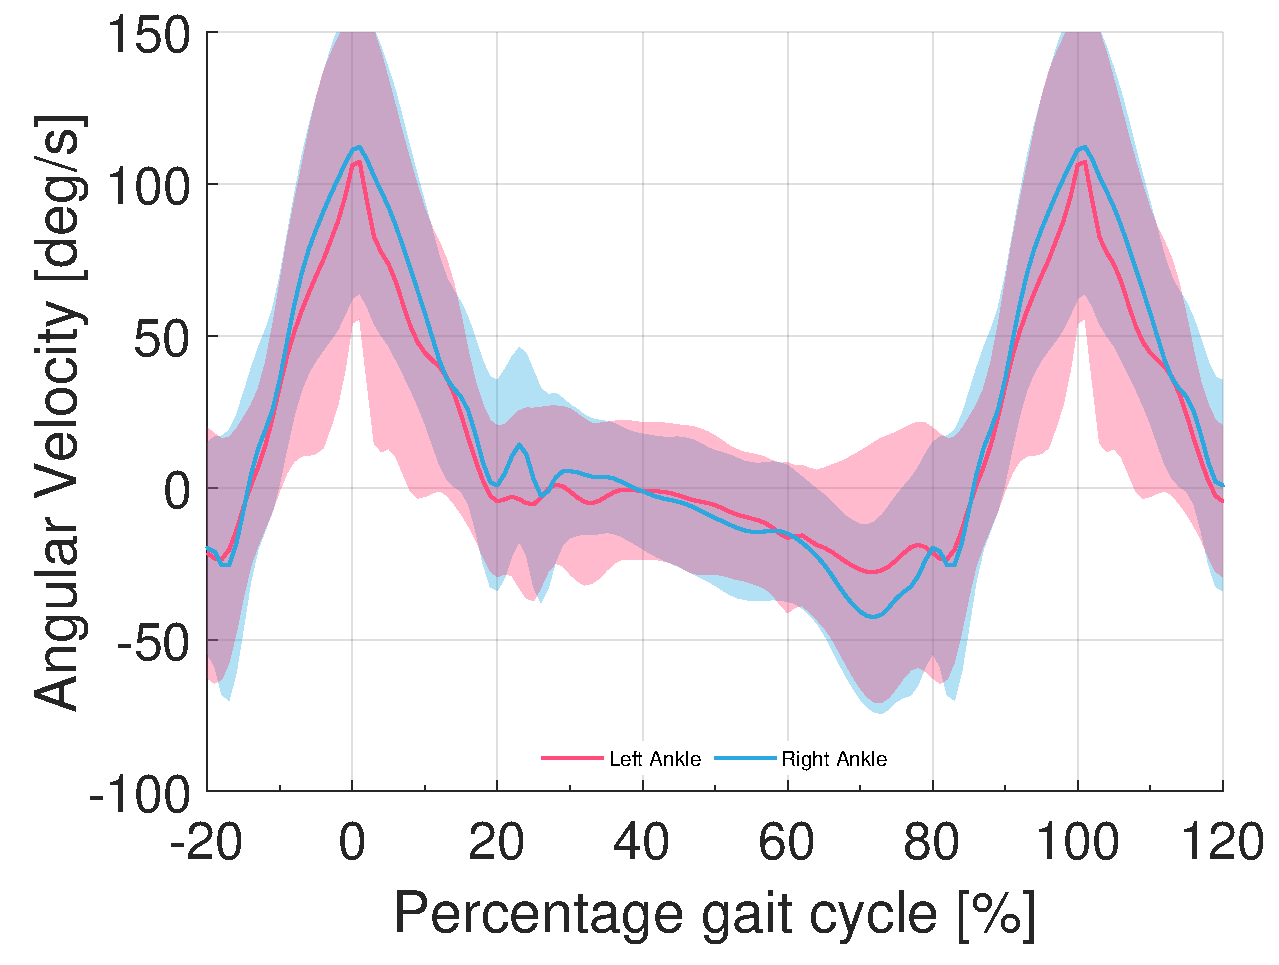
\includegraphics[width=\linewidth]{content/5-Personalisation/Gyro_Trends_For_Targets/ch5_gait_trends_subject_01_activity_walking.pdf}\end{subfigure} & \begin{subfigure}[b]{0.275\textwidth}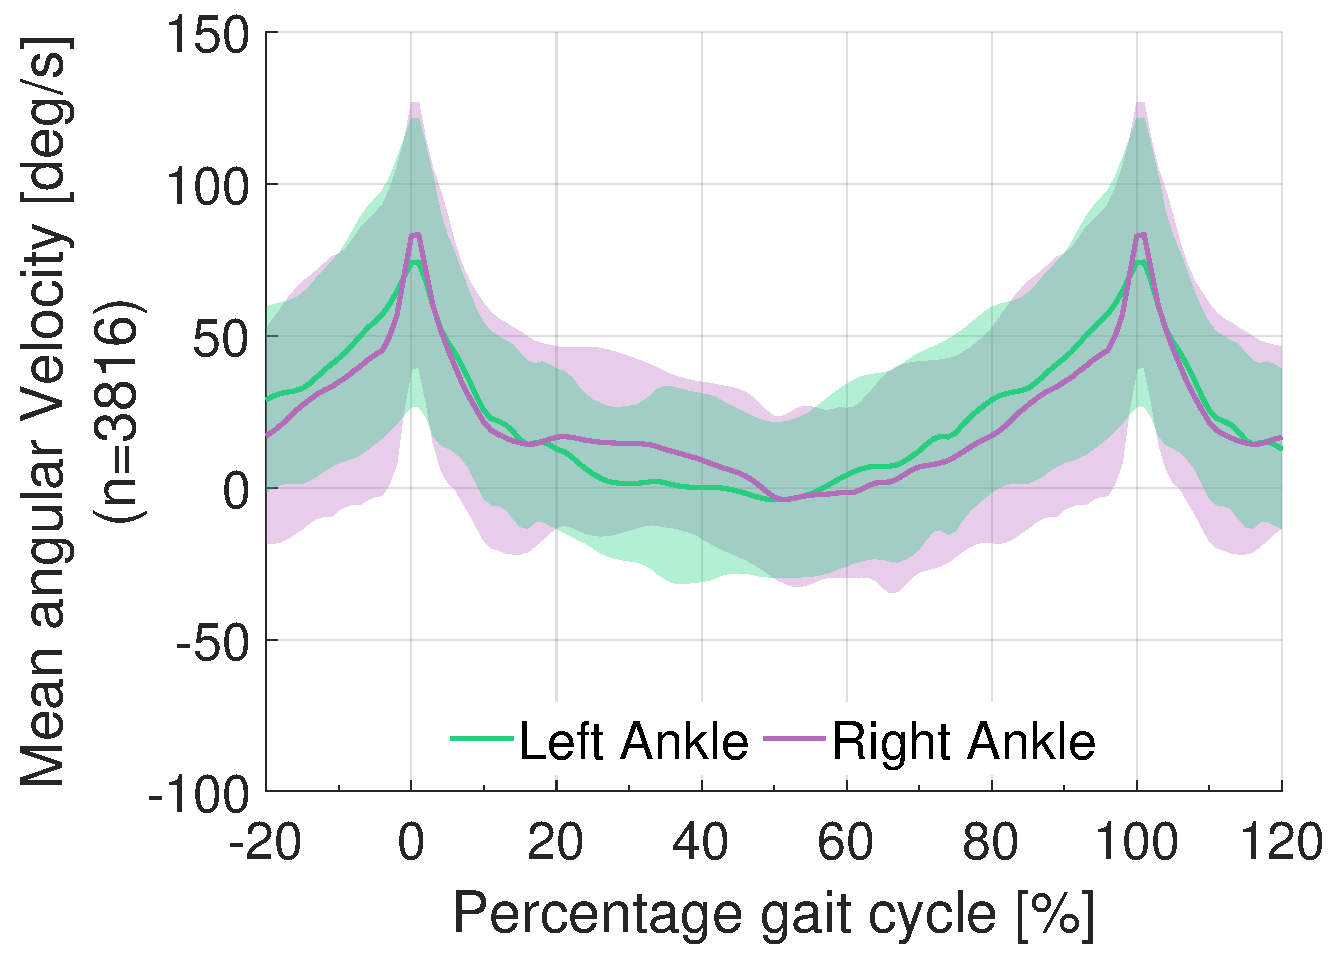
\includegraphics[width=\linewidth]{content/5-Personalisation/Gyro_Trends_For_Targets/ch5_gait_trends_subject_03_activity_walking.pdf}\end{subfigure} &
        \begin{subfigure}[b]{0.275\textwidth}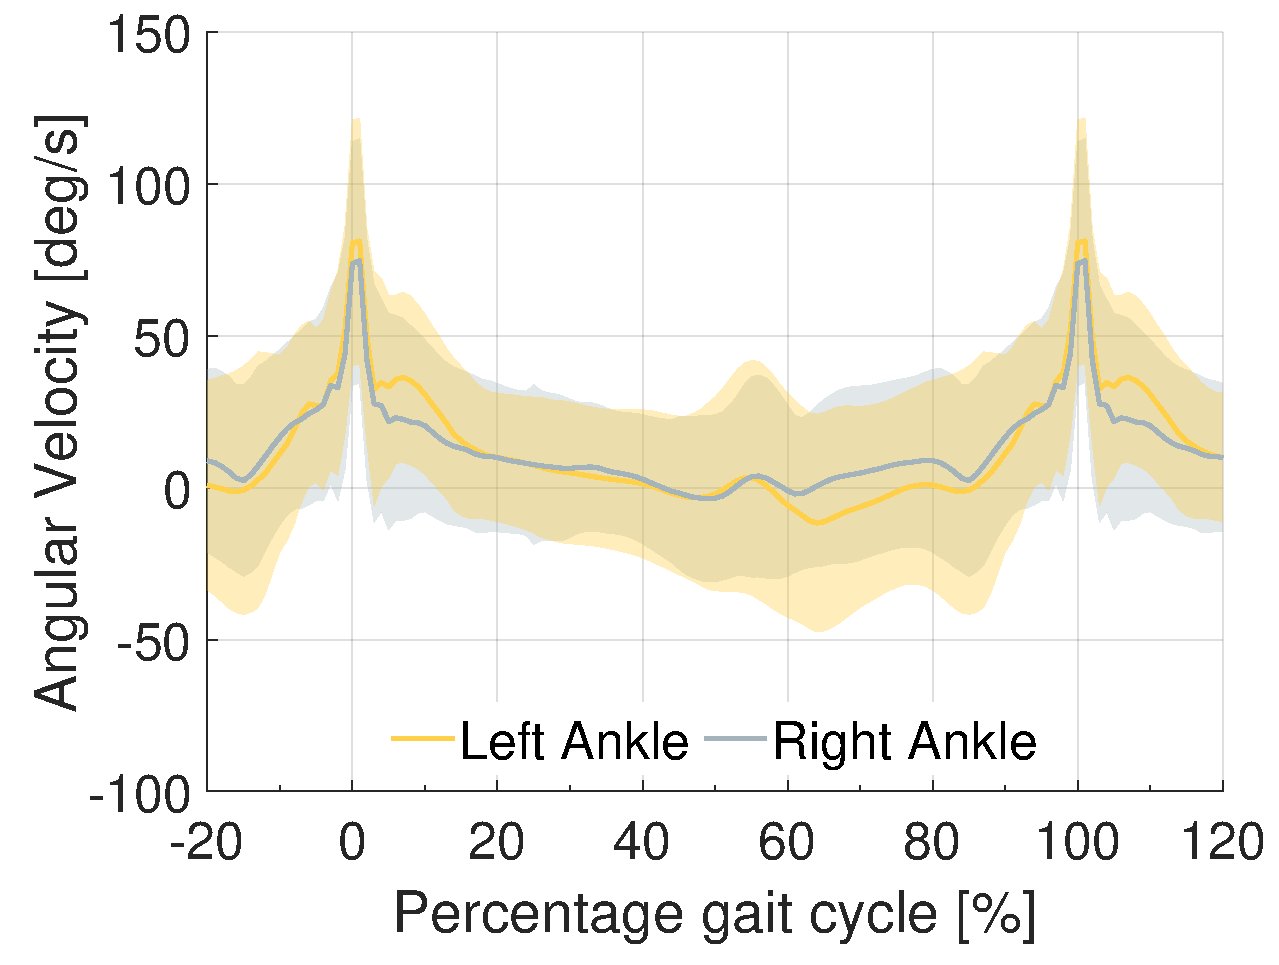
\includegraphics[width=\linewidth]{content/5-Personalisation/Gyro_Trends_For_Targets/ch5_gait_trends_subject_09_activity_walking.pdf}\end{subfigure} \\
        \rotatebox{90}{~\quad \textbf{\glsentrylong{ra}}} & 
        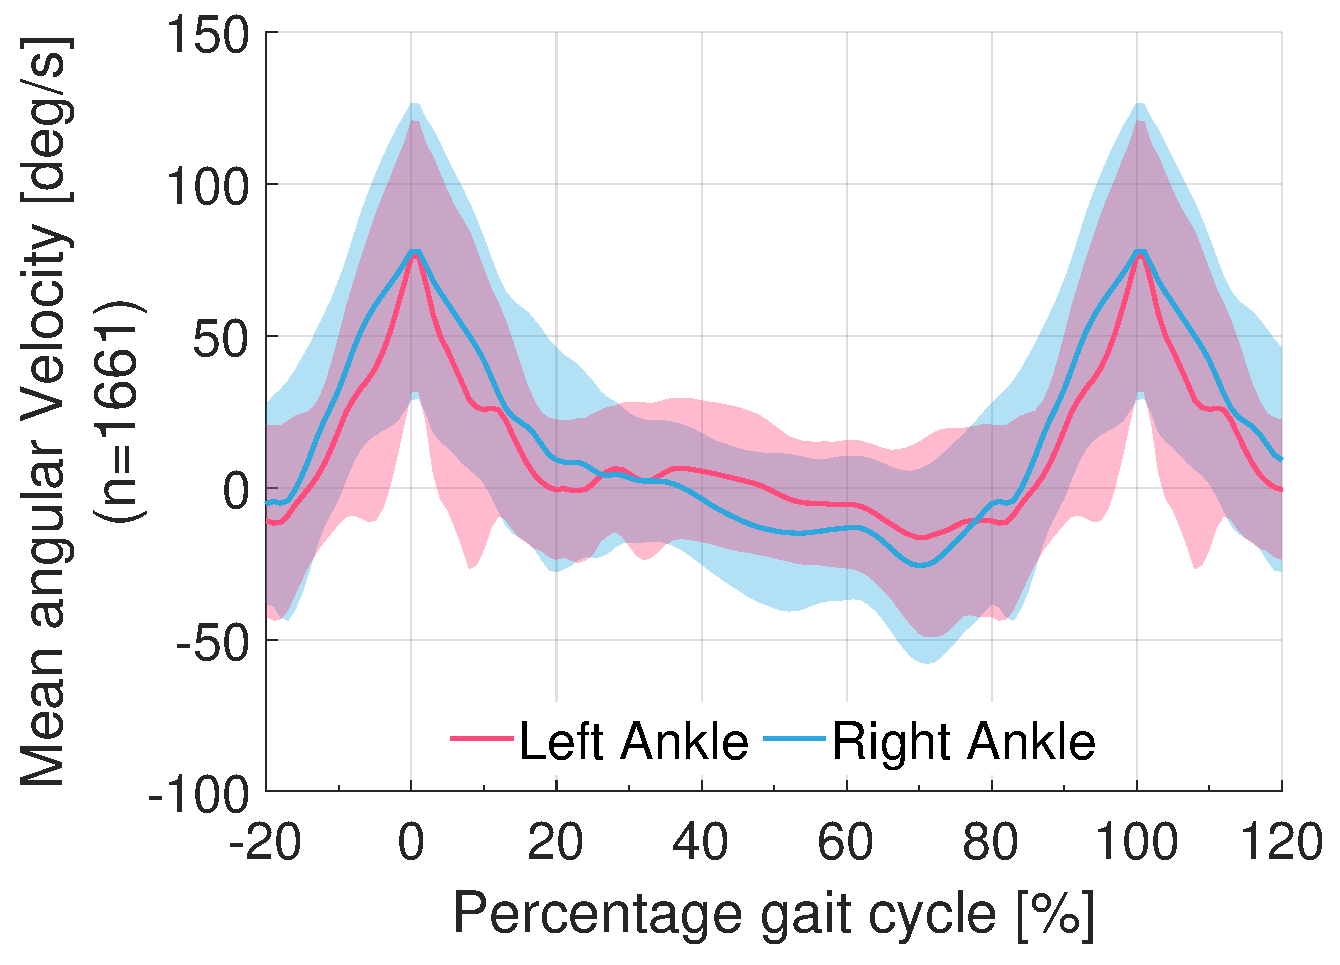
\includegraphics[width=0.275\linewidth]{content/5-Personalisation/Gyro_Trends_For_Targets/ch5_gait_trends_subject_01_activity_ramp_up.pdf} & 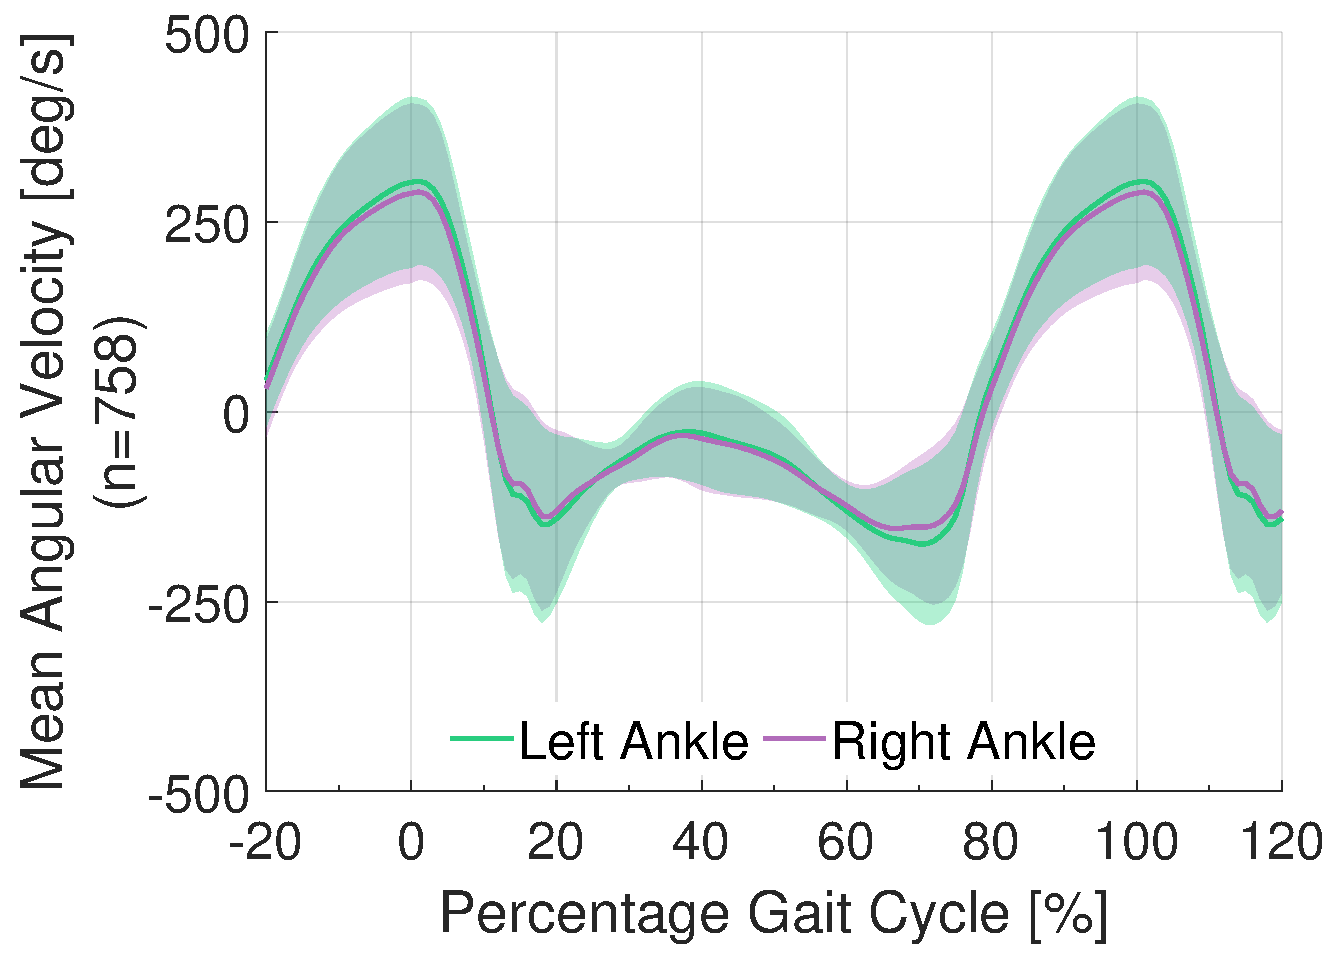
\includegraphics[width=0.275\linewidth]{content/5-Personalisation/Gyro_Trends_For_Targets/ch5_gait_trends_subject_03_activity_ramp_up.pdf} &
        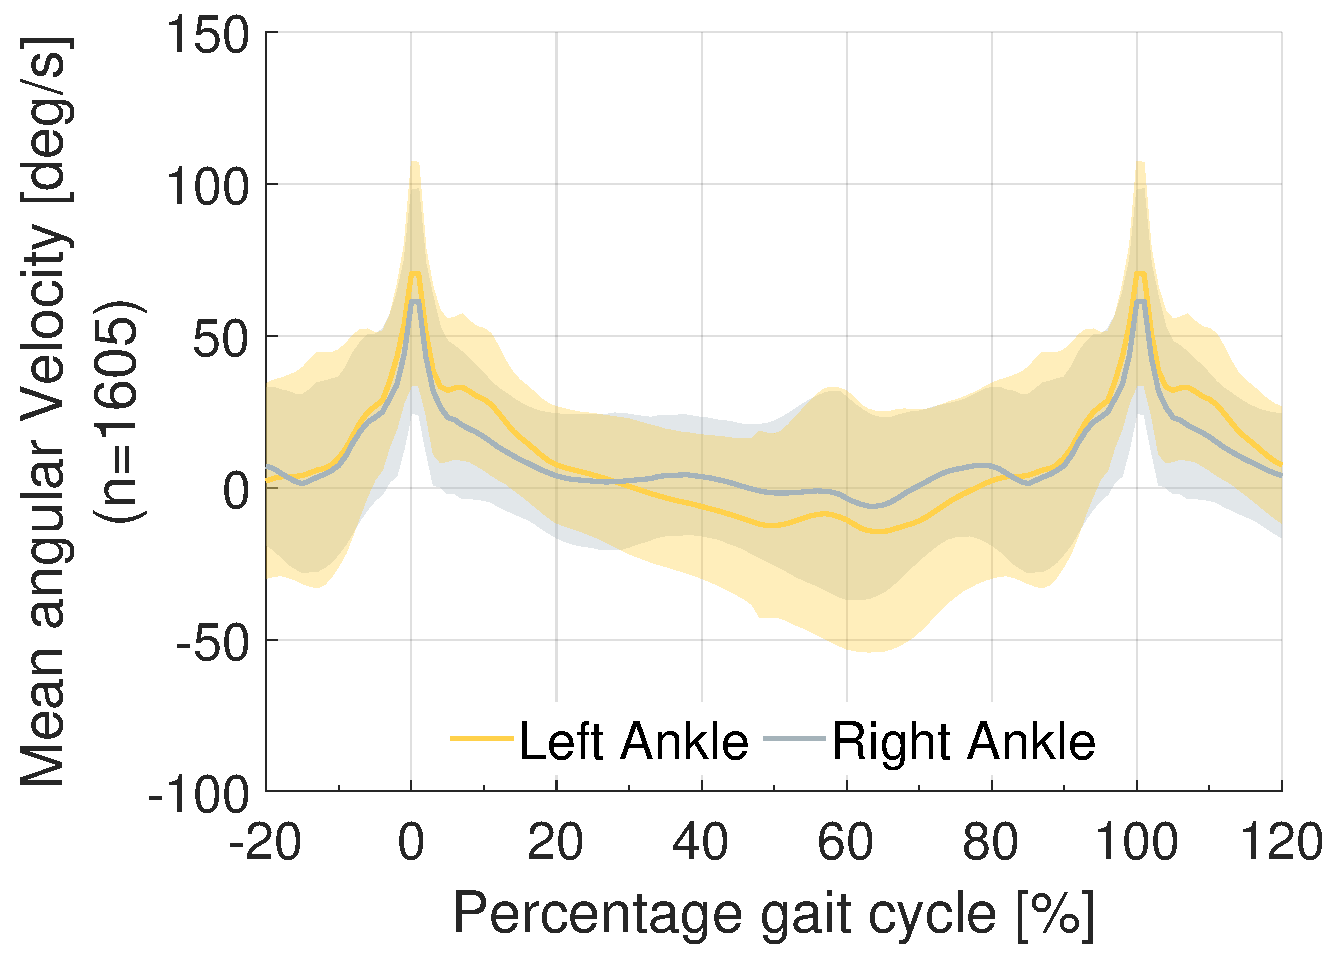
\includegraphics[width=0.275\linewidth]{content/5-Personalisation/Gyro_Trends_For_Targets/ch5_gait_trends_subject_09_activity_ramp_up.pdf} \\
        \rotatebox{90}{\quad \textbf{\glsentrylong{rd}}} & 
        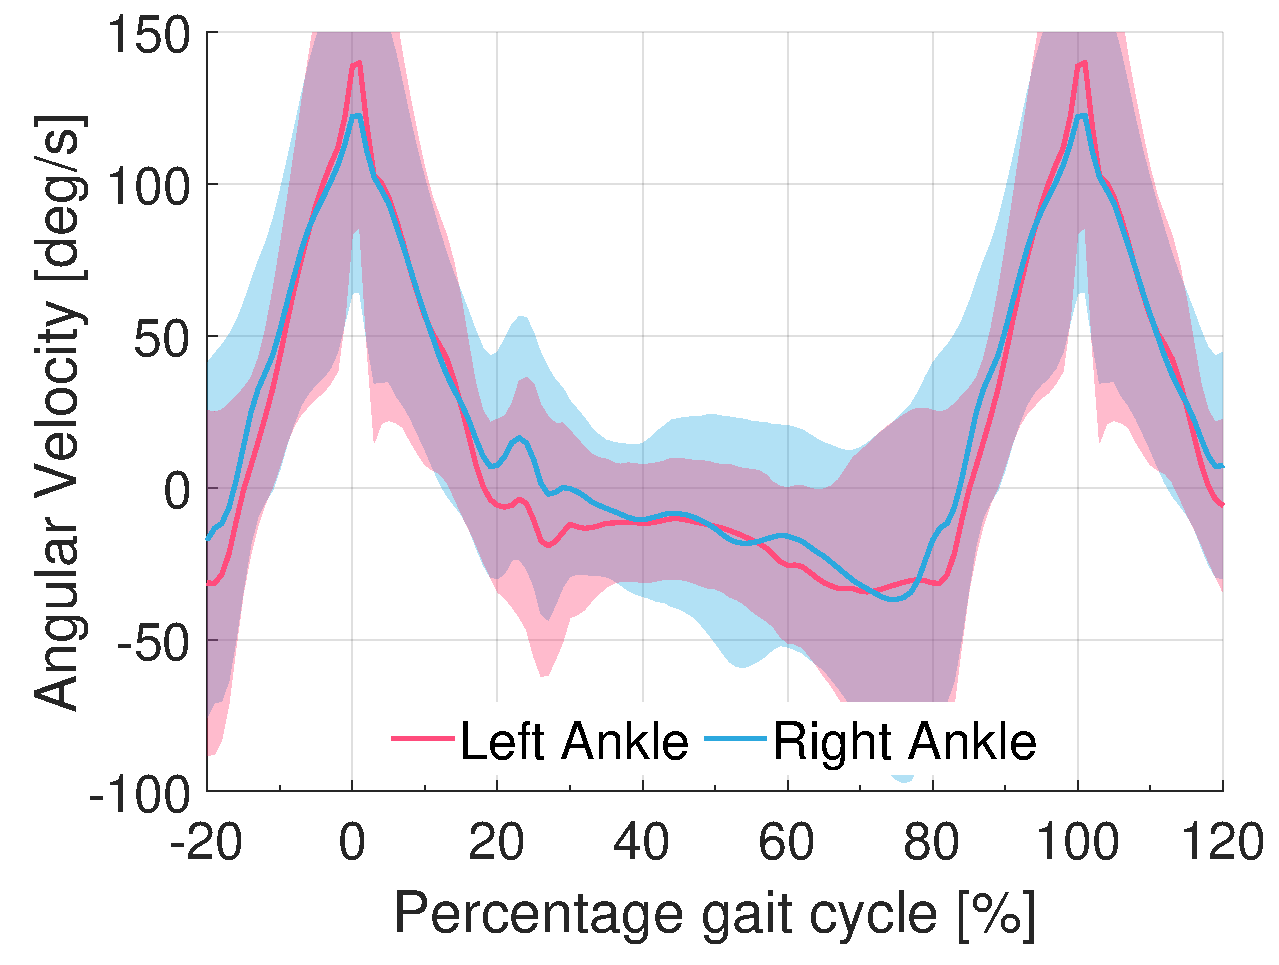
\includegraphics[width=0.275\linewidth]{content/5-Personalisation/Gyro_Trends_For_Targets/ch5_gait_trends_subject_01_activity_ramp_down.pdf} & 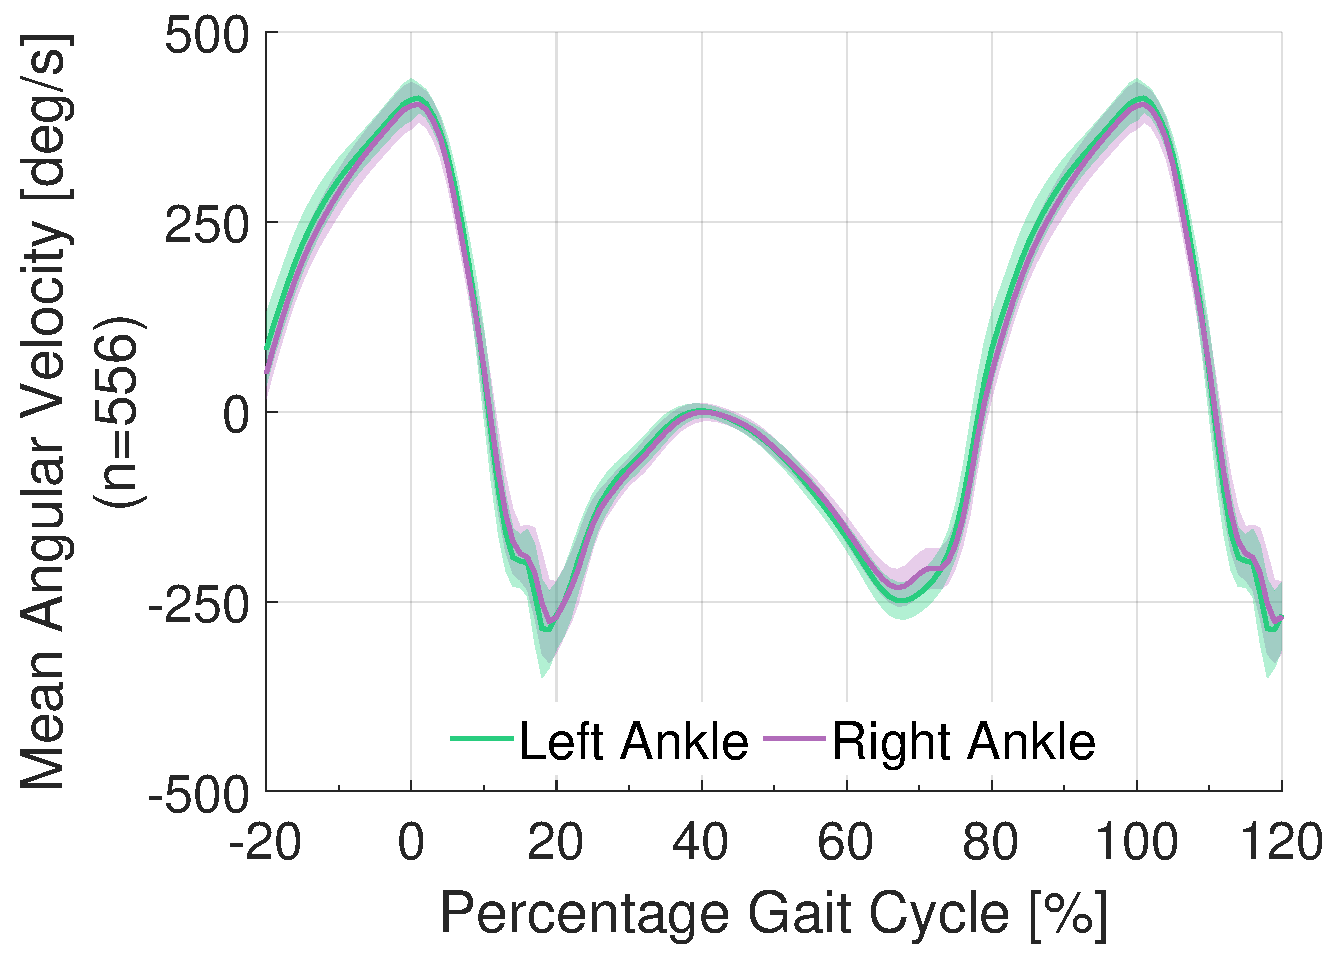
\includegraphics[width=0.275\linewidth]{content/5-Personalisation/Gyro_Trends_For_Targets/ch5_gait_trends_subject_03_activity_ramp_down.pdf} &
        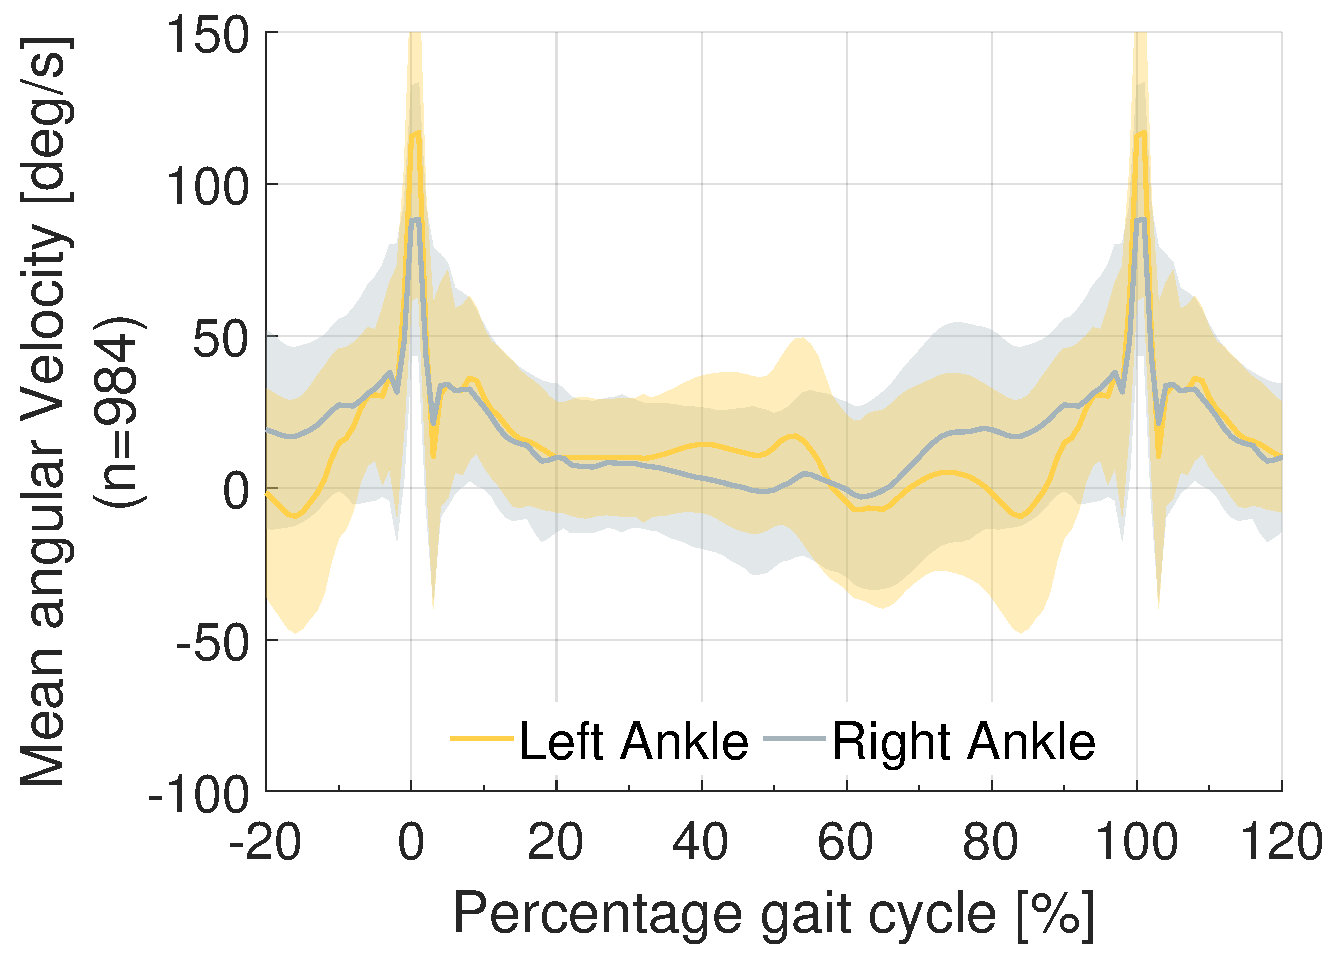
\includegraphics[width=0.275\linewidth]{content/5-Personalisation/Gyro_Trends_For_Targets/ch5_gait_trends_subject_09_activity_ramp_down.pdf} \\
        \rotatebox{90}{~\quad \textbf{\glsentrylong{sa}}} & 
        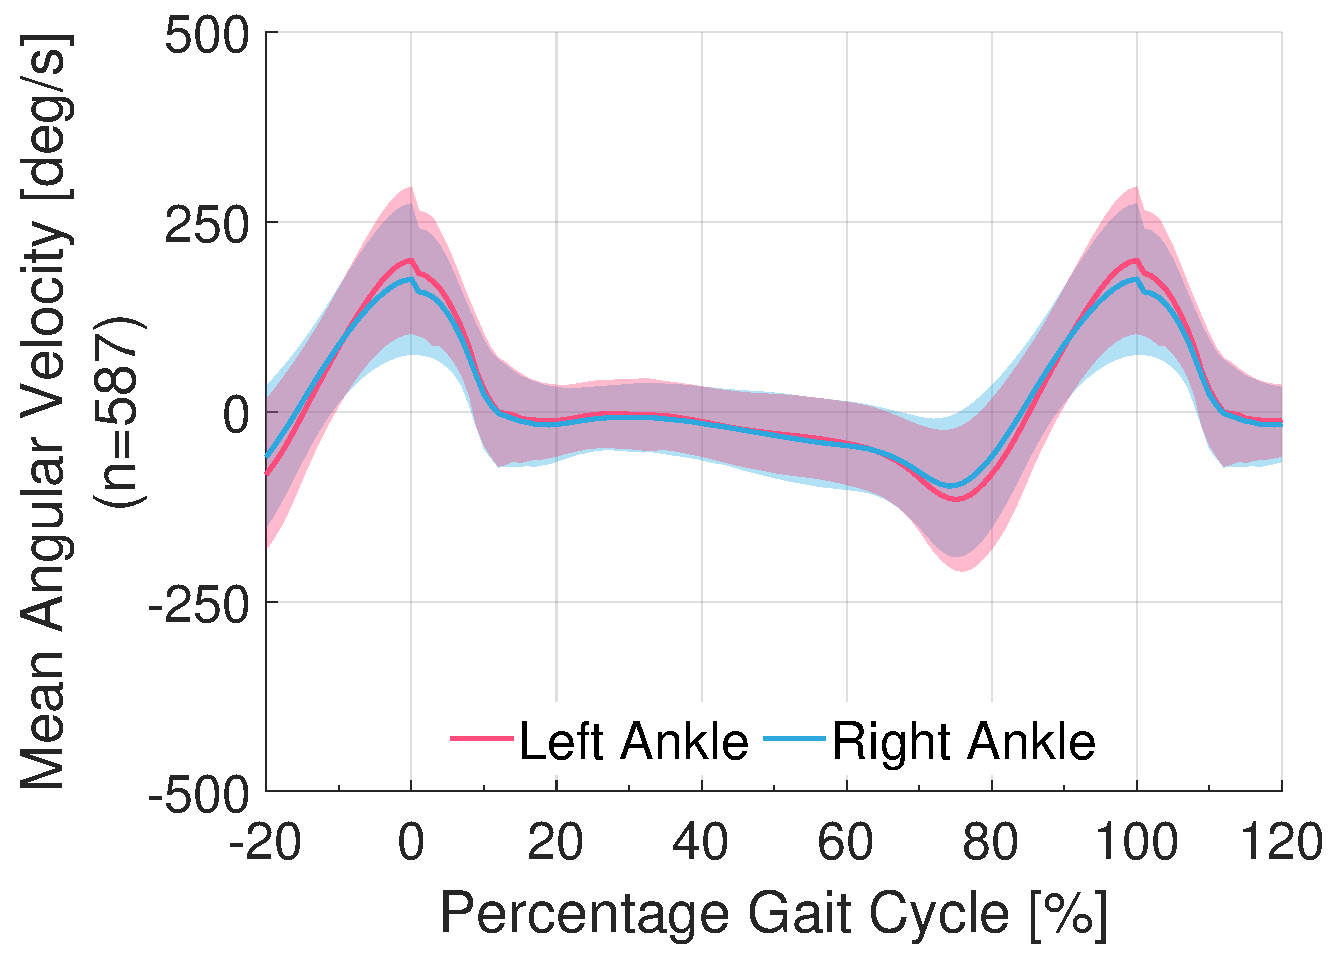
\includegraphics[width=0.275\linewidth]{content/5-Personalisation/Gyro_Trends_For_Targets/ch5_gait_trends_subject_01_activity_stair_up.pdf} & 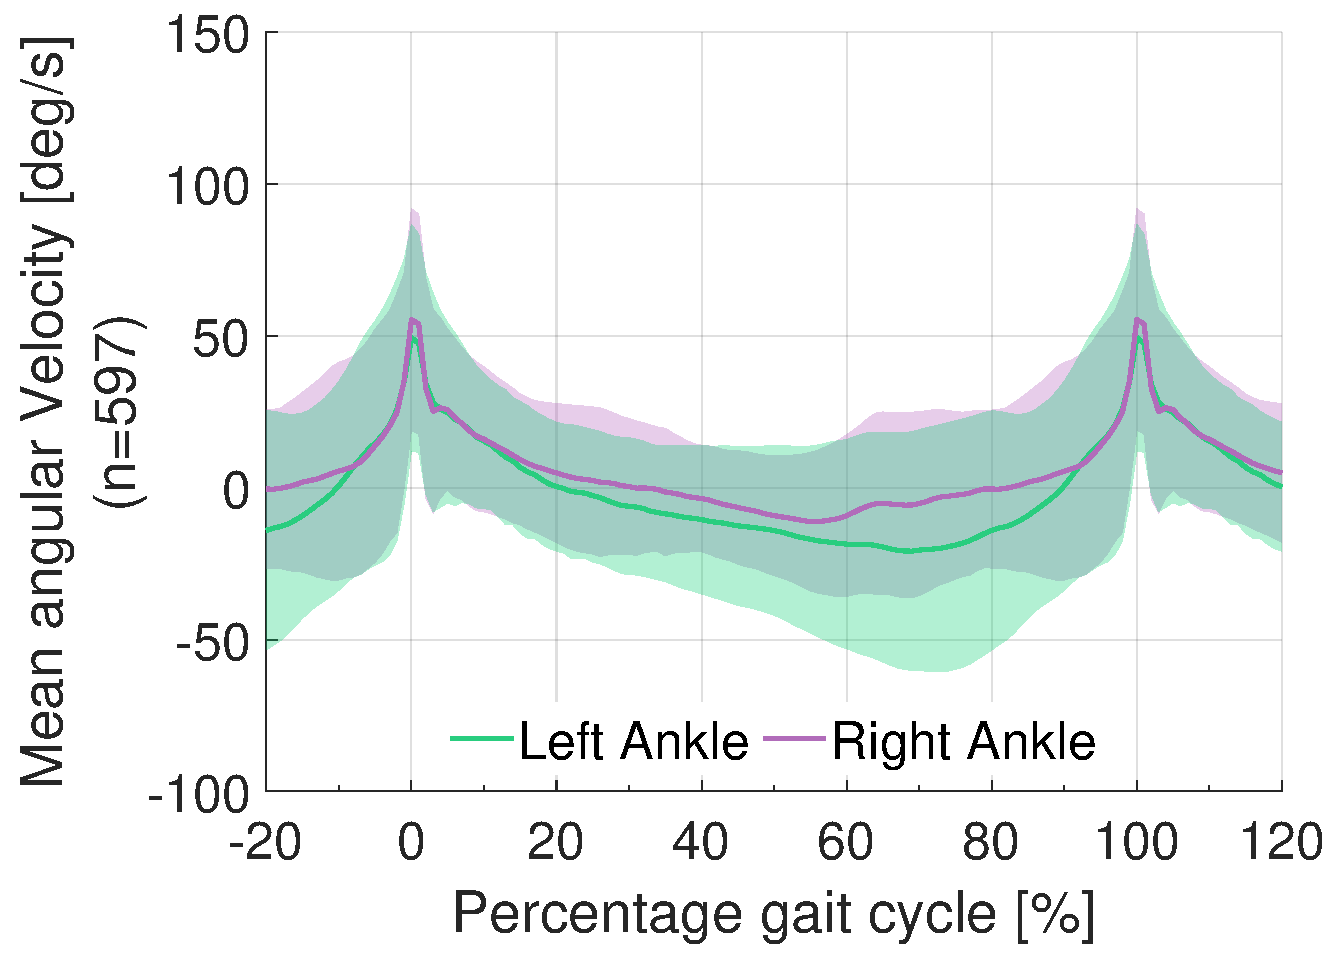
\includegraphics[width=0.275\linewidth]{content/5-Personalisation/Gyro_Trends_For_Targets/ch5_gait_trends_subject_03_activity_stair_up.pdf} &
        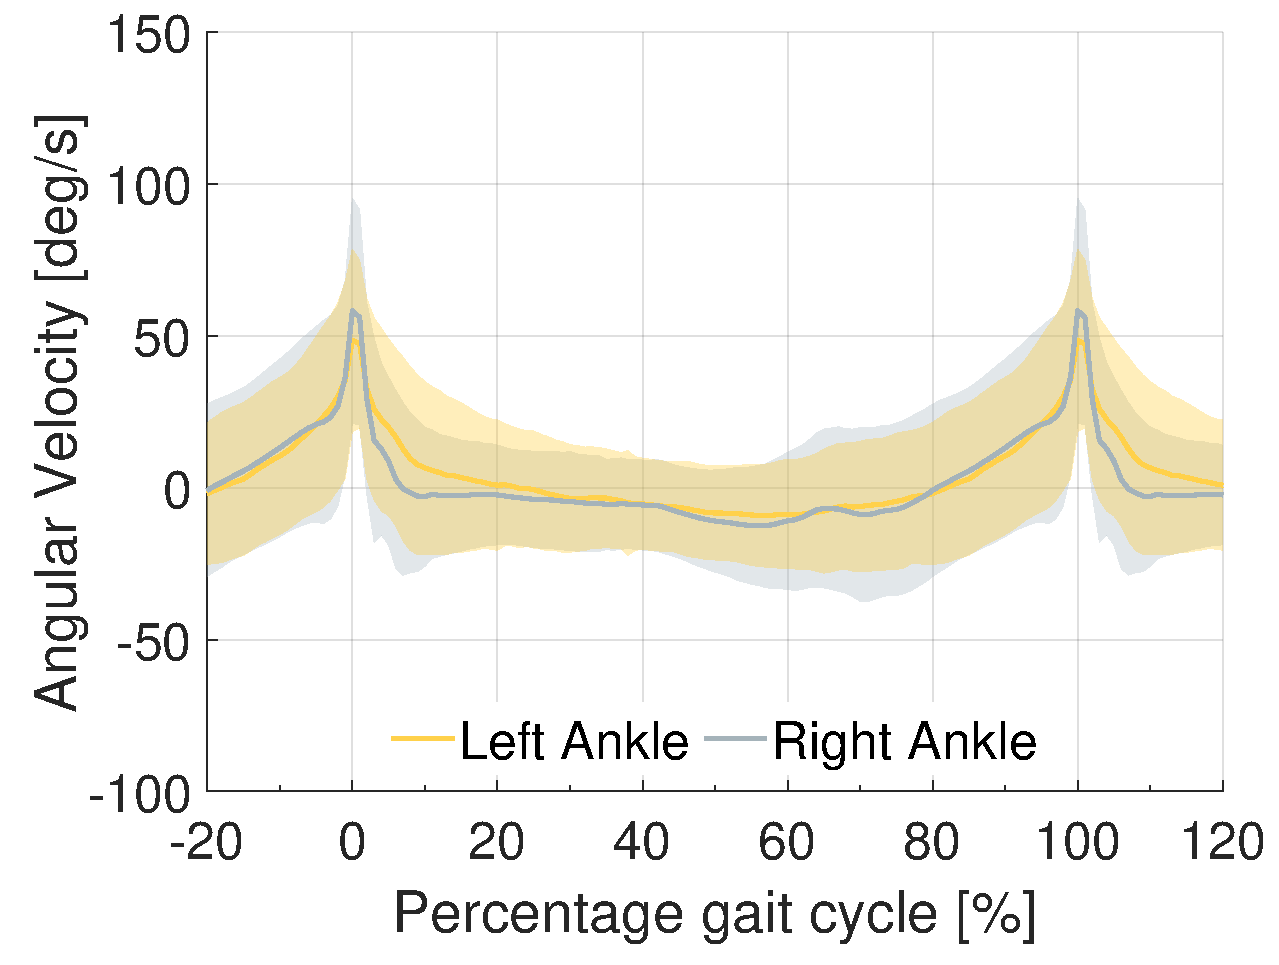
\includegraphics[width=0.275\linewidth]{content/5-Personalisation/Gyro_Trends_For_Targets/ch5_gait_trends_subject_09_activity_stair_up.pdf} \\
        \rotatebox{90}{\quad \textbf{\glsentrylong{sd}}} & 
        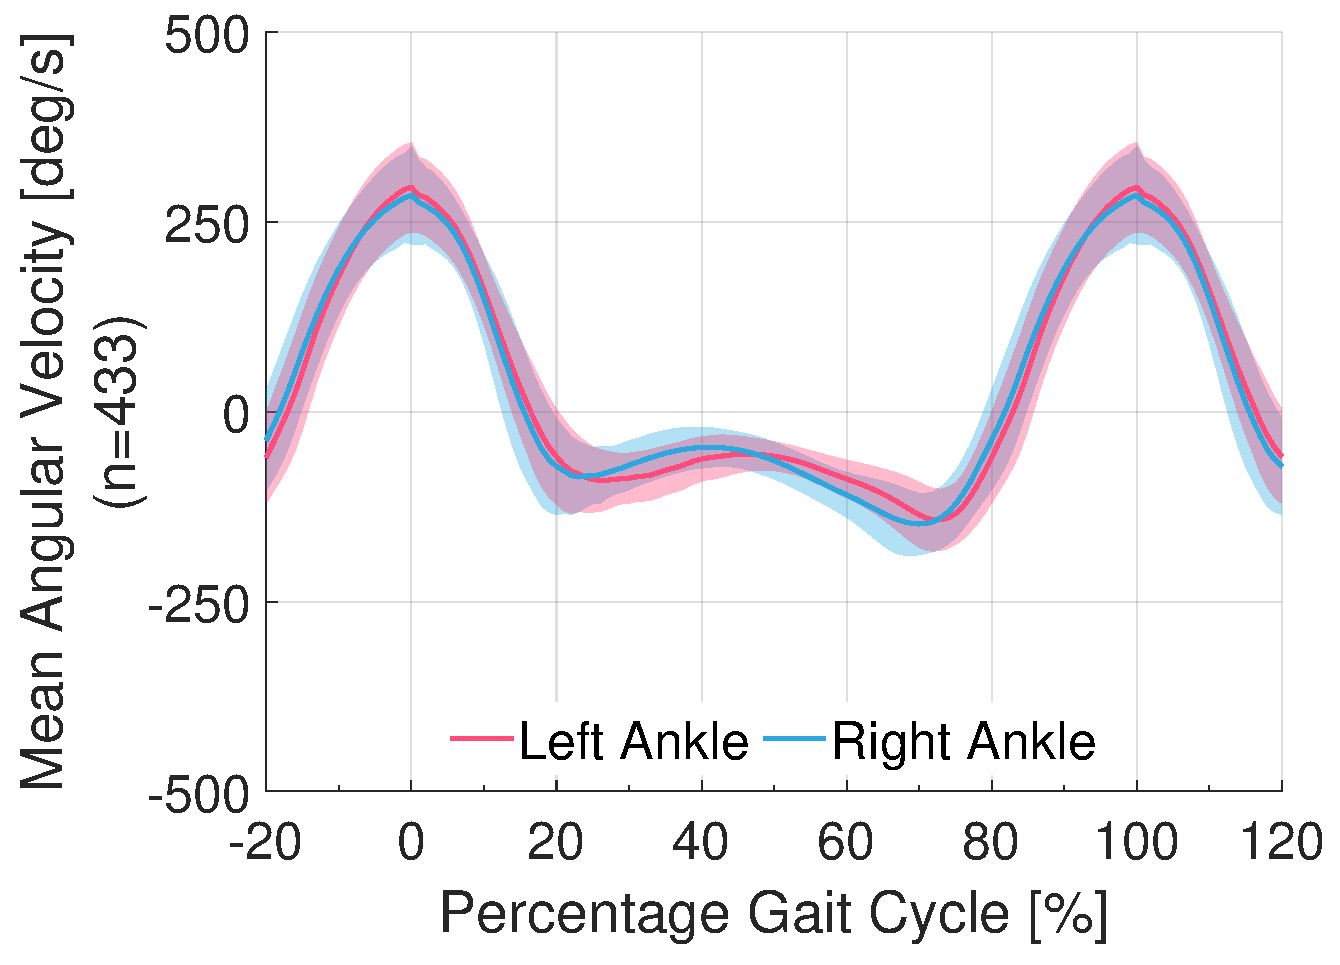
\includegraphics[width=0.275\linewidth]{content/5-Personalisation/Gyro_Trends_For_Targets/ch5_gait_trends_subject_01_activity_stair_down.pdf} & 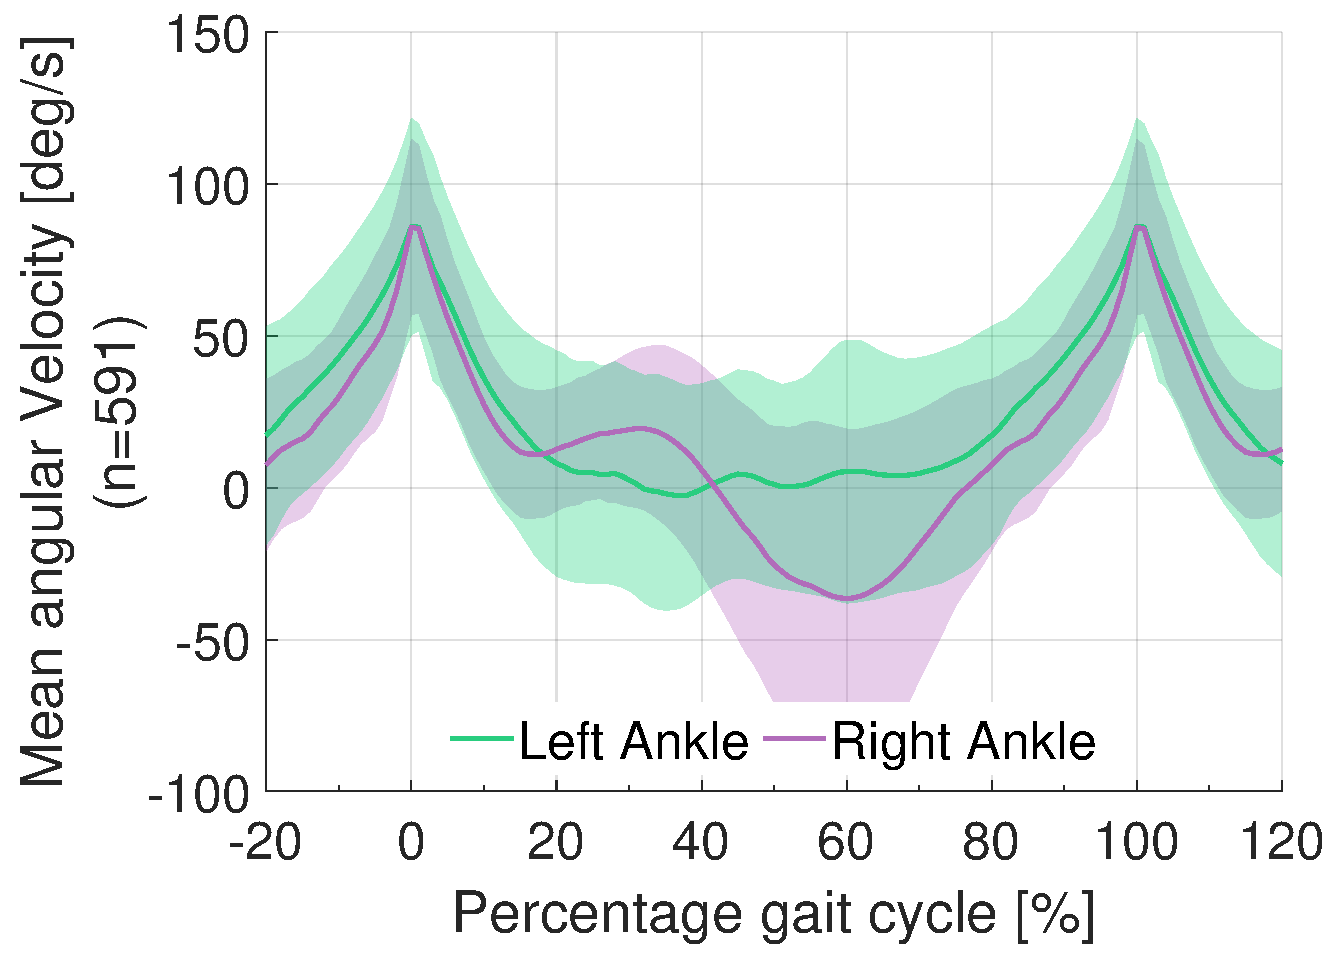
\includegraphics[width=0.275\linewidth]{content/5-Personalisation/Gyro_Trends_For_Targets/ch5_gait_trends_subject_03_activity_stair_down.pdf} &
        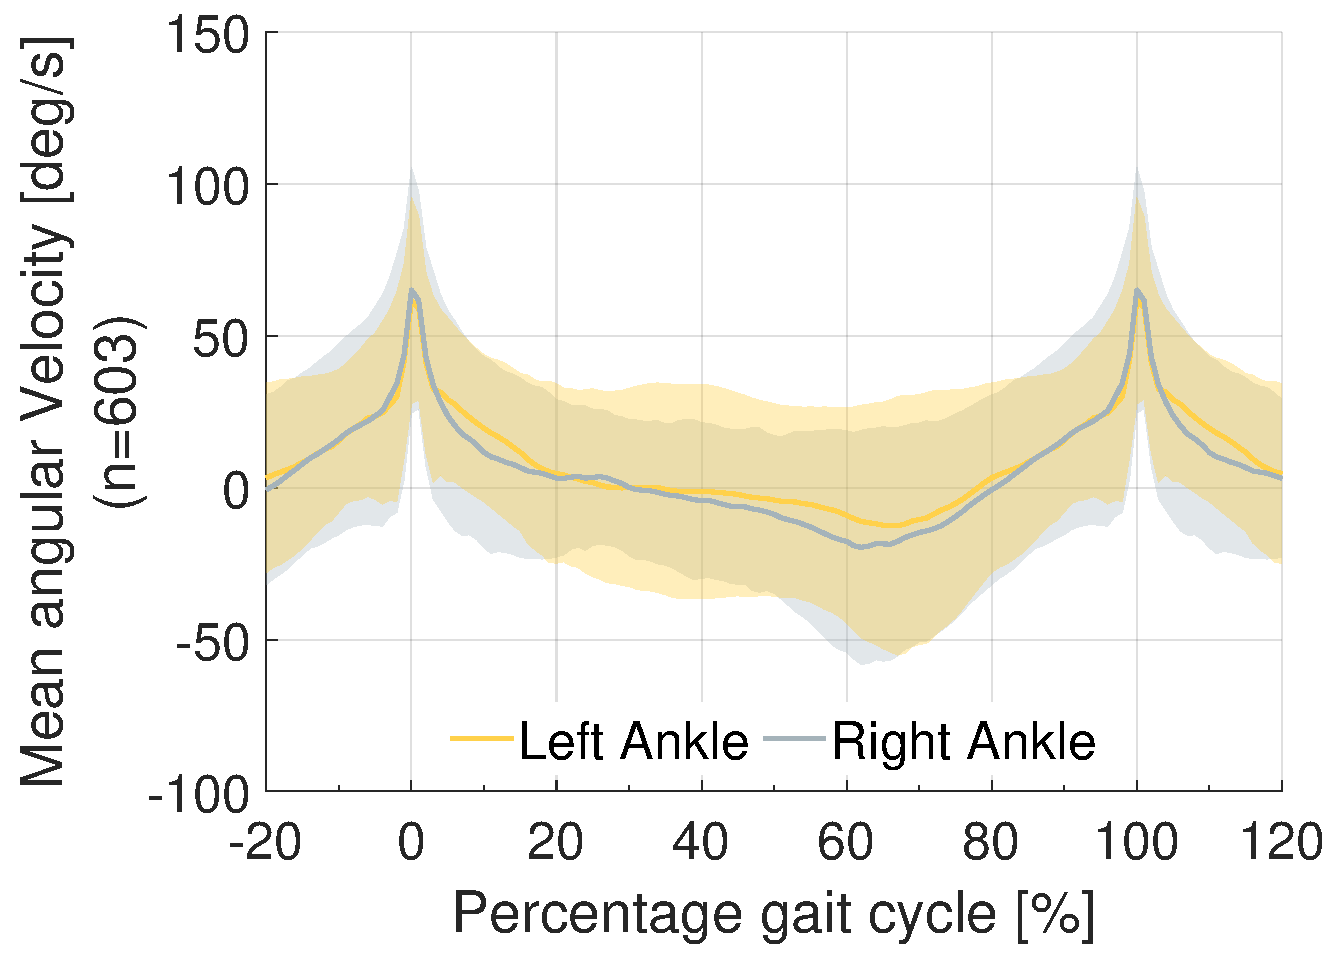
\includegraphics[width=0.275\linewidth]{content/5-Personalisation/Gyro_Trends_For_Targets/ch5_gait_trends_subject_09_activity_stair_down.pdf} \\
    \end{tabular}
    \centering
    \caption[Angular velocity of the shank in the Saggital Plane during different activities for the three target subject]{Angular velocity of the shank in the Saggital Plane during different activities for the three target subject. The solid line shows the mean angular velocity for all steps recorded for each activity. The filled area represents the standard deviation. 0\% gait cycle is taken as peak swing for simplicity of calculation. The red, green and yellow lines are for the left ankles of Subjects 1, 3 and 9 respectively. The blue, purple and grey lines show the right ankles of Subjects 1, 3 and 9 respectively.}
    \label{fig:personalistaion_target_subjects_gyro_trends}
\end{figure}

\subsection{Data Division}
The HAR data set is made of a series of continuous recordings which may cover multiple different activities and environments. Developing an effective method for dividing this data will be critical to demonstrating the effectiveness of personalisation.

It is highly likely to suffer from poor distribution of classes since activities such as walking are far more prevalent than climbing stairs. As \acrshort{ml} methods perform best using balanced data sets, this must be corrected. Additionally, in order for the test set to represent a novel environment, the training data sets should ideally not include any data from the same environment. Therefore each unique episode should only be used once across the training and test data sets. Finally the data division method should allow for multiple repeatable unique sets to be constructed to allow for cross-validation of performance. Achieving all these requirements means that the recordings cannot simply be divided by time.

The proposed approach is to divide the continuous data of each subject into episodes, each containing one continuous period of activity. Episodes can then be combined to form the three independent data sets. The three sets required are training - a set of examples from which the model can learn; validation - used to evaluate the generalisation performance during training; and test used to evaluate the generalisation performance after training.

Each episode is only used once, any excess episodes are discarded. To balance the number of classes, excess windows are discarded randomly from all episodes. To produce cross-validation sets the starting order of the episodes can be shuffled. Figure \ref{fig:methods-per-episode-data-division} illustrates the process of forming the three data sets.

\begin{figure}[hbt]
     \centering
     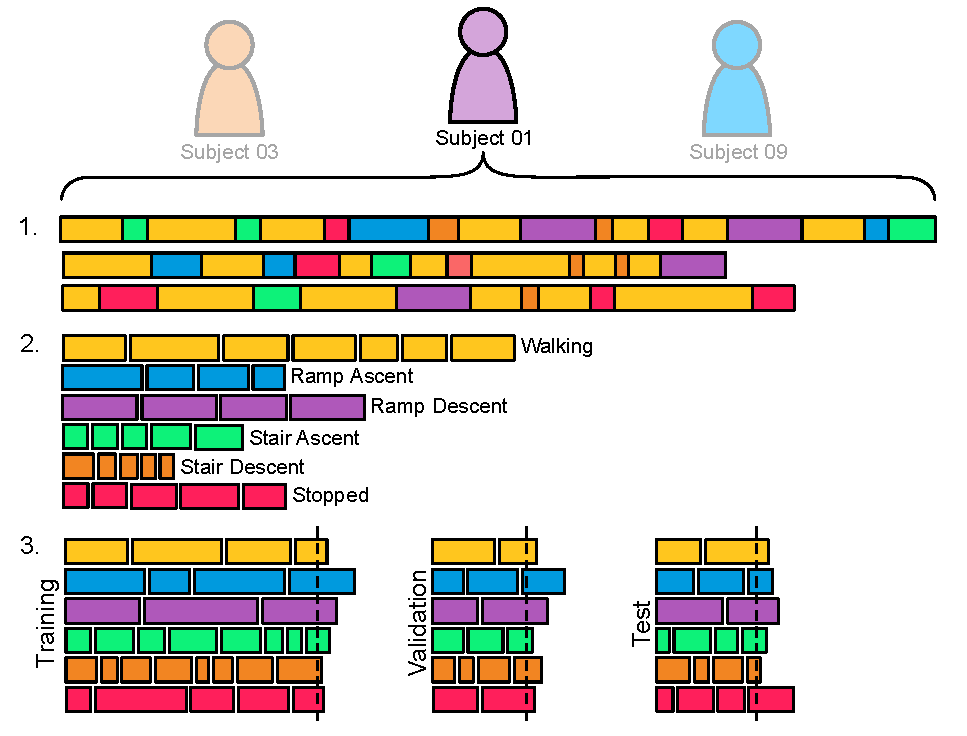
\includegraphics[width=0.9\textwidth]{content/5-Personalisation/Episode_Division.pdf}
     \caption[Per-episode data division]{Per-episode data division. Step 1 -- Labelled data files for a single subject are loaded. Step 2 -- Episodes of the same activity are grouped together. Step 3 -- Training, Validation and Test sets are formed by stacking episodes until the required window quantity reached.}
     \label{fig:methods-per-episode-data-division}
 \end{figure}
 
%BOOKMARK (SM) - PROOF READ UP TO HERE
For all experiments the test sets will contain 5000 windows of target data. Training/validation set will vary in length. For conciseness the number of training windows will be presented as the sum of both training and validation windows. These will always be in the ratio 70:30. 

Each experiment will be repeated multiple time with episodes randomly shuffled between each to improve statistical certainty. The shuffling will be repeatable and test data will always be drawn first to ensure a consistent test set.

The time in seconds can be calculated using Equation \ref{eqn:episode_set_length_seconds}, where $T$ is total set length in seconds, $f_s$ is the sampling frequency, $s_k$ is the window skip value, $n_w$ is the number of windows, $l_w$ is the window size, and $n_e$ is the number of episodes included in the set.

\begin{equation}
    T = \frac{1}{f_s}(s_k n_w + l_w n_e)
    \label{eqn:episode_set_length_seconds}
\end{equation}

Calculating the actual quantity of data used in seconds is non-trivial as some windows may be dropped during class balancing. Assuming no windows are dropped and only one episode is used 5000 windows uses a minimum of 151 seconds for each class. $l_w$ set to 128, $f_s$ set to 100Hz, and $s_k$ equal to three.

%--------------------------------
% Machine learning methods
\subsection{Machine Learning Methods}
Two personalisation methods will be evaluated -- data supplementation and transfer learning. These will be compared against two baselines, a model trained using only target training data, and a general subject agnostic model.

The data supplementation technique will mix source and target data to produce a larger training set. This will then be used to train a new classifier from scratch. The additional data will be selected randomly without attempting to match similar subjects. The amount of both source and target data will be varied to investigate the impact of both.

The transfer learning approach will fine-tuned a set of base general models using data from a target subject. The base models will be generated by training a model from scratch using the full source data excluding the three target subjects. Five base model will be produced, by randomly shuffling the training and validation.

Personalisation will be performed by additional training using just target data. The amount of target training data used will be varied to asses the impact of this of classification performance. Three different training configurations will be tested, each configuration will vary by which layers are trained. For the first configuration all layers will be fine-tuned, the second and third method will train only the \acrshort{lstm} and dense layers respectively.

The same \acrshort{lstm} architecture will be used throughout all experiments shown in Figure \ref{fig:ch5_illustration_of_base_LSTM_model}. This is the same architecture as used in Chapter \ref{chp:lstm-general}. The first has an \acrshort{lstm} layer than takes a 128 x 6 input of raw \acrshort{imu} data. The \acrshort{lstm} layer can be a varying number of units wide but will always be 128 units long. The full output of this layer is then passed to a dense late fusion layer before been passed through a \acrshort{relu} classifier. TensorFlow allocates 4992 parameters to a 32 unit 128 long LSTM layer and 24582 parameters to the Dense layer.

\begin{figure}[htbp]
    \centering
    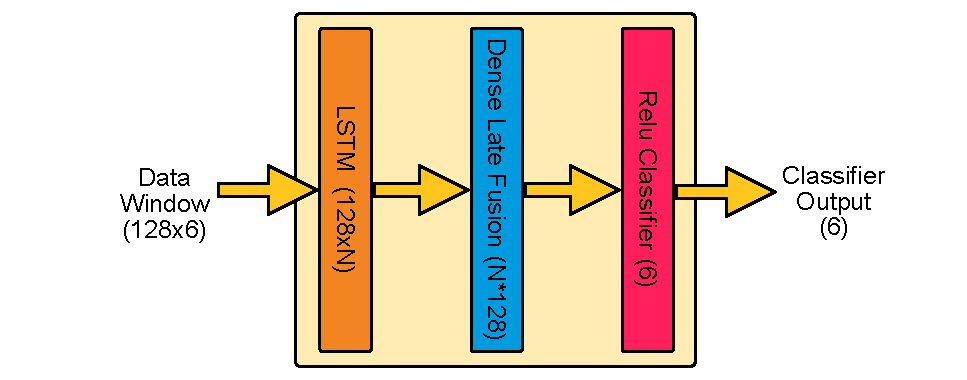
\includegraphics[width=0.8\textwidth]{content/5-Personalisation/ch5_lstm_architecture.pdf}
    \caption[Illustration of \glsentryshort{lstm} machine learning model architecture]{Illustration of \acrshort{lstm} machine learning model architecture}
    \label{fig:ch5_illustration_of_base_LSTM_model}
\end{figure}

All training will be undertake using the same methods as described in Chapter \ref{chp:lstm-general}. The full set of windows will be passed thought the training systems in mini-batches of 100 windows. After every epoch the validation set will be used to evaluate the performance of the model. When the categorical loss of the validation set stagnates for more than 3 epochs training will be stopped. All training hyper-parameters were tune empirically.

Model performance will be assessed primarily by the classification accuracy using the unseen test data set. Additionally measures include the number of epochs, training time and quantity of training data required. These will aim in determining the computationally/data efficient. By using comparison against the baselines it will be possible to determine if these methods are of benefit.


%-------------------------------------------------------------------------------
\section{Baseline Model Performance}
\label{sec:personalisation-baseline-model-results}
To determine if personalisation has resulted in an improvement a performance baseline is required. Two baselines will be generated for each target subject. These will be the accuracy of a general model for the target, and the accuracy of a model trained using only target data. If performance of the personalisation methods do not exceed the baselines there is no benefit in them. The performance of both baselines is presented within this section.

% Performance of the trained general models with no fine-tuning
For the first baseline the classification accuracy of the general models when presented with the test data sets was evaluated. The average accuracy of the five models was $75.0\%\pm2.3$ for Subject 1, $63.9\%\pm2.9$ for Subject 3 and $77.4\%\pm5.1$ for Subject 9. The confusion matrices for each subject is presented in Table \ref{tab:ch5-general-model-confusion-matrix}. Performance is averaged across the five general models and five test sets. Each cell contains the percentage of total predictions of each class.

Table \ref{tab:ch5-general-model-confusion-matrix} shows that each target subject struggles at different classes. This is as you would expect given the likely differences in gait characteristics.

% Confusion matrix for general model
\begin{table}[p]
    \centering
    \caption[Confusion matrix of a general model presented with target subject test data]{Confusion matrix of a general model presented with target subject test data. Columns represent the prediction labels and the rows represent the real labels. Each value represent the percentage of total predictions of that class. (\acrfull{ra}, \acrfull{rd}, \acrfull{sa}, \acrfull{sd})}
    \label{tab:ch5-general-model-confusion-matrix}
    \begin{subtable}{\textwidth}
    \caption{Subject 1}
    \begin{tabularx}{\textwidth}{ccYYYYYY}
        \noalign{\hrule height 1.5pt}
         & & \multicolumn{6}{c}{\textbf{Predicted Classes}} \\
         \hline
         & & WALK & \glsentryshort{ra} & \glsentryshort{rd} & \glsentryshort{sa} & \glsentryshort{sd} & STOP \\
         \multirow{6}{*}{\rotatebox{90}{\textbf{True Classes}}} 
         & WALK               & 37.9 & 26.9 & 24.5 & 0.1 & 6.2 & 6.3 \\
         & \glsentryshort{ra} & 57.9 & 65.3 & 1.2 & 1.0 & 0.2 & 0.0 \\
         & \glsentryshort{rd} & 2.4 & 0.9 & 72.8 & 0.0 & 3.7 & 0.5 \\
         & \glsentryshort{sa} & 0.5 & 5.9 & 0.0 & 98.6 & 1.3 & 2.0 \\
         & \glsentryshort{sd} & 1.1 & 0.8 & 1.5 & 0.2 & 88.6 & 5.8 \\
         & STOP               & 0.2 & 0.3 & 0.0 & 0.0 & 0.0 & 85.4 \\
         \noalign{\hrule height 1.5pt} \\
    \end{tabularx}
    \end{subtable}
    \begin{subtable}{\textwidth}
    \caption{Subject 3}
    \begin{tabularx}{\textwidth}{ccYYYYYY}
        \noalign{\hrule height 1.5pt}
         & & \multicolumn{6}{c}{\textbf{Predicted Classes}} \\
         \hline
         & & WALK & \glsentryshort{ra} & \glsentryshort{rd} & \glsentryshort{sa} & \glsentryshort{sd} & STOP \\
         \multirow{6}{*}{\rotatebox{90}{\textbf{True Classes}}} 
         & WALK               & 27.4 & 29.5 & 1.7 & 4.3 & 5.4 & 19.6 \\
         & \glsentryshort{ra} & 40.3 & 70.2 & 1.0 & 0.2 & 0.1 & 2.3 \\
         & \glsentryshort{rd} & 31.6 & 0.2 & 94.3 & 0.5 & 8.2 & 0.9 \\
         & \glsentryshort{sa} & 0.4 & 0.1 & 0.3 & 94.9 & 0.7 & 0.9 \\
         & \glsentryshort{sd} & 0.3 & 0.0 & 2.7 & 0.1 & 85.6 & 0.0 \\
         & STOP               & 0.0 & 0.0 & 0.0 & 0.0 & 0.0 & 76.3 \\
         \noalign{\hrule height 1.5pt} \\
    \end{tabularx}
    \end{subtable}
    \begin{subtable}{\textwidth}
    \caption{Subject 9}
    \begin{tabularx}{\textwidth}{ccYYYYYY}
        \noalign{\hrule height 1.5pt}
         & & \multicolumn{6}{c}{\textbf{Predicted Classes}} \\
         \hline
         & & WALK & \glsentryshort{ra} & \glsentryshort{rd} & \glsentryshort{sa} & \glsentryshort{sd} & STOP \\
         \multirow{6}{*}{\rotatebox{90}{\textbf{True Classes}}} 
         & WALK               & 59.6 & 8.5 & 10.7 & 0.5 & 9.3 & 1.3 \\
         & \glsentryshort{ra} & 13.3 & 89.2 & 0.2 & 14.6 & 2.5 & 1.0 \\
         & \glsentryshort{rd} & 17.7 & 0.0 & 84.3 & 0.0 & 15.7 & 0.0 \\
         & \glsentryshort{sa} & 4.7 & 1.7 & 0.0 & 78.3 & 1.2 & 2.1 \\
         & \glsentryshort{sd} & 4.7 & 0.5 & 4.8 & 0.5 & 71.4 & 2.9 \\
         & STOP               & 0.1 & 0.0 & 0.0 & 6.0 & 0.0 & 92.6 \\
         \noalign{\hrule height 1.5pt} \\
    \end{tabularx}
    \end{subtable}
\end{table}

To determine a baseline for models trained with only target training data LSTM models of different shapes were trained using increasing amounts of target data. Figure \ref{fig:ch5_bespoke_mode_classification} shows the classification performance for each of subject using different quantities of target data windows for 6, 16, 32 and 64 unit \acrshort{lstm} networks. The full data tables are available in Appendix \ref{chp:tables-of-results} Section \ref{sec:appendix-a-model-performance-bespoke}.

% Confusion matrix for bespoke model
\begin{table}[p]
    \centering
    \caption[confusion matrix for a bespoke \acrshort{lstm} model presented with target subject test data]{confusion matrix for a bespoke \acrshort{lstm} model presented with target subject test data. The 32 unit \acrshort{lstm} model was trained with 15000 target data window. Columns represent the prediction labels and the rows represent the real labels. Each value represent the percentage of total predictions of that class. (\acrfull{ra}, \acrfull{rd}, \acrfull{sa}, \acrfull{sd})}
    \label{tab:ch5-bespoke-model-confusion-matrix}
    \begin{subtable}{\textwidth}
    \caption{Subject 1}
    \begin{tabularx}{\textwidth}{ccYYYYYY}
        \noalign{\hrule height 1.5pt}
         & & \multicolumn{6}{c}{\textbf{Predicted Classes}} \\
         \hline
         & & WALK & \glsentryshort{ra} & \glsentryshort{rd} & \glsentryshort{sa} & \glsentryshort{sd} & STOP \\
         \multirow{6}{*}{\rotatebox{90}{\textbf{True Classes}}} 
         & WALK               & 71.3 & 20.6 & 18.1 & 0.4 & 1.9 & 2.7 \\
         & \glsentryshort{ra} & 25.9 & 72.4 & 0.0 & 0.0 & 0.0 & 0.0 \\
         & \glsentryshort{rd} & 1.2 & 0.0 & 80.0 & 0.2 & 6.2 & 0.0 \\
         & \glsentryshort{sa} & 0.9 & 5.6 & 0.2 & 92.9 & 5.2 & 0.2 \\
         & \glsentryshort{sd} & 0.8 & 1.2 & 1.7 & 4.5 & 86.7 & 1.7 \\
         & STOP               & 0.1 & 0.1 & 0.0 & 2.0 & 0.1 & 95.4 \\
         \noalign{\hrule height 1.5pt} \\
    \end{tabularx}
    \end{subtable}
    \begin{subtable}{\textwidth}
    \caption{Subject 3}
    \begin{tabularx}{\textwidth}{ccYYYYYY}
        \noalign{\hrule height 1.5pt}
         & & \multicolumn{6}{c}{\textbf{Predicted Classes}} \\
         \hline
         & & WALK & \glsentryshort{ra} & \glsentryshort{rd} & \glsentryshort{sa} & \glsentryshort{sd} & STOP \\
         \multirow{6}{*}{\rotatebox{90}{\textbf{True Classes}}} 
         & WALK               & 50.3 & 3.3 & 4.2 & 0.2 & 4.1 & 3.1 \\
         & \glsentryshort{ra} & 32.3 & 52.1 & 0.3 & 0.0 & 0.0 & 0.0 \\
         & \glsentryshort{rd} & 16.5 & 43.5 & 92.1 & 0.1 & 0.5 & 0.0 \\
         & \glsentryshort{sa} & 0.5 & 0.8 & 0.2 & 99.2 & 1.5 & 1.0 \\
         & \glsentryshort{sd} & 0.2 & 0.2 & 3.1 & 0.5 & 94.0 & 0.1 \\
         & STOP               & 0.1 & 0.0 & 0.0 & 0.0 & 0.1 & 95.7 \\
         \noalign{\hrule height 1.5pt} \\
    \end{tabularx}
    \end{subtable}
    \begin{subtable}{\textwidth}
    \caption{Subject 9}
    \begin{tabularx}{\textwidth}{ccYYYYYY}
        \noalign{\hrule height 1.5pt}
         & & \multicolumn{6}{c}{\textbf{Predicted Classes}} \\
         \hline
         & & WALK & \glsentryshort{ra} & \glsentryshort{rd} & \glsentryshort{sa} & \glsentryshort{sd} & STOP \\
         \multirow{6}{*}{\rotatebox{90}{\textbf{True Classes}}} 
         & WALK               & 90.4 & 7.6 & 6.3 & 2.0 & 2.7 & 0.0 \\
         & \glsentryshort{ra} & 2.2 & 82.5 & 0.1 & 1.4 & 0.1 & 0.0 \\
         & \glsentryshort{rd} & 5.6 & 7.4 & 85.1 & 2.1 & 8.8 & 0.0 \\
         & \glsentryshort{sa} & 1.0 & 1.7 & 0.6 & 92.8 & 4.7 & 0.1 \\
         & \glsentryshort{sd} & 0.8 & 0.6 & 8.0 & 1.6 & 83.4 & 0.7 \\
         & STOP               & 0.1 & 0.2 & 0.0 & 0.2 & 0.4 & 99.2 \\
         \noalign{\hrule height 1.5pt} \\
    \end{tabularx}
    \end{subtable}
\end{table}

% Classification performance
\begin{figure}[p]
    \centering
    \begin{subfigure}[b]{\textwidth}
        \centering
        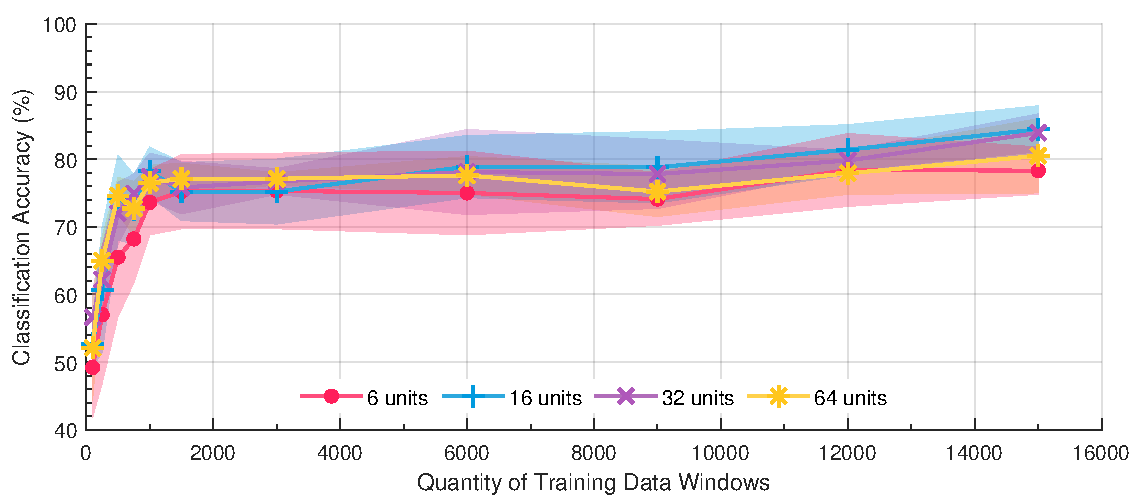
\includegraphics[width=\textwidth]{content/5-Personalisation/Bespoke_Target/ch5_bespoke_target_model_subject_1.pdf}
        \caption{Subject 1}
        \label{fig:ch5_6_unit_bespoke_model}
    \end{subfigure}
    \begin{subfigure}[b]{\textwidth}
        \centering
        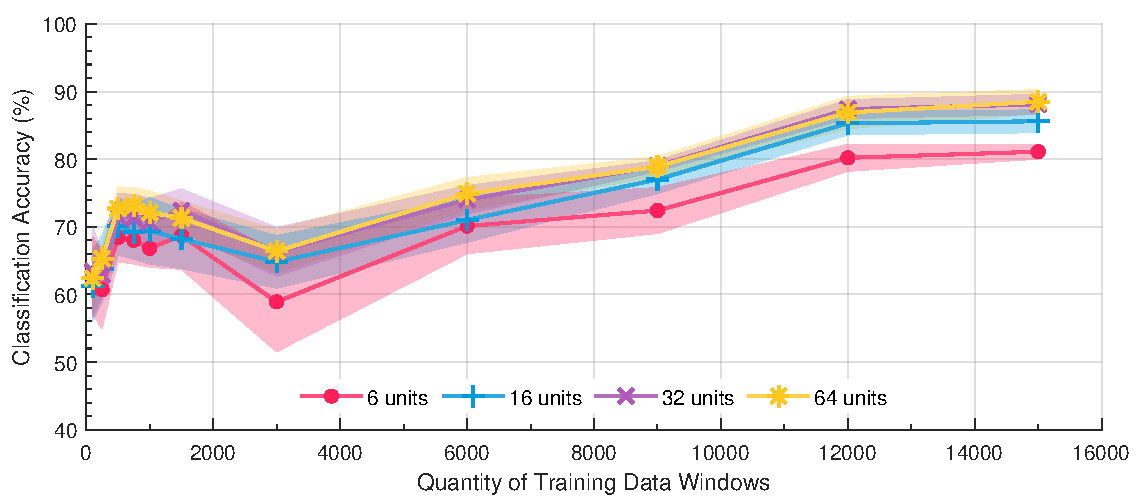
\includegraphics[width=\textwidth]{content/5-Personalisation/Bespoke_Target/ch5_bespoke_target_model_subject_3.pdf}
        \caption{Subject 3}
        \label{fig:ch5_16_unit_bespoke_model}
    \end{subfigure}
    \caption[Classification performance of different size \glsentryshort{lstm} networks trained with varying amount of target subject data]{Classification performance of different size \acrshort{lstm} networks trained with varying amount of target subject data. The solid lines represent the mean of all models trained, the filled area represents the standard deviation $(n=10)$. Each line show the classification performance for a different number of \acrshort{lstm} units. The red dot is 6 units, blue plus 16, purple cross 32 and yellow asterisk 64.}
    \label{fig:ch5_bespoke_mode_classification}
\end{figure}
\begin{figure}[t]\ContinuedFloat
    \begin{subfigure}[b]{\textwidth}
        \centering
        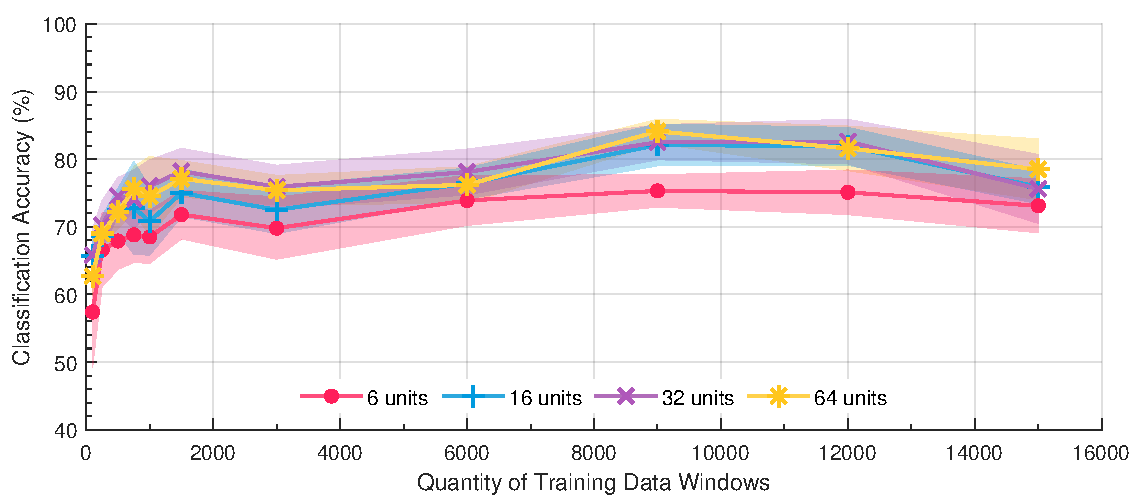
\includegraphics[width=\textwidth]{content/5-Personalisation/Bespoke_Target/ch5_bespoke_target_model_subject_9.pdf}
        \caption{Subject 9}
        \label{fig:ch5_32_unit_bespoke_model}
    \end{subfigure}
    \caption[]{Classification performance of different size \acrshort{lstm} networks trained with varying amount of target subject data (Cont.).}
\end{figure}

%BOOKMARK - (FS) REWRITTEN UP TO HERE
The maximum performance achieved was $84.4\%$ for Subject 1, $88.5\%$ for Subject 3, and $82.6\%$ for Subject 9. This was achieved at 15000 windows for Subjects 1 and 3 but 9000 samples for Subject 9. It's not clear why performance decreased after this point. Performance of the general model is exceeded at around 1500 windows.

The fastest rate of performance improvement was seen early on, from 100 to 1500 data windows. Beyond this there was a more gradual increase in performance. It appears that performance would have continued to improve the maximum number of windows tested. Indicating further data would still improve performance. 

Standard deviation reduced with increasing quantities of data windows indicating more consistent performance across all test sets as as the model was exposed to more data.

The baseline model took on average 8 epochs to train with a 95\textsuperscript{th} percentile of 13

Increasing the number of units in general improved classification performance. This levels off at 32 units. Only the 6 unit model appears to have insufficient learning capacity. Increasing the number of units also reduced the number of epochs required to train the models. Therefore 32 units is likely a good candidate for future models.

The reduction in performance at 3000 samples for Subject 3 is likely due to model exposure to a new environment of data. Performance recovers with increasing amounts of data. Subject 9 also experiences similar drops in performance.

%Why is the model not achieving better performance?
An assessment of where classification errors are occurring can be made by looking at the confusion matrices. Table \ref{tab:ch5-bespoke-model-confusion-matrix} shows confusion matrices for the three targets classifiers created using 15000 training windows. Performance is averaged across the five bespoke models test sets. Each cell contains the percentage of total predictions of each class.

The confusion matrices show that the stop class achieves the highest accuracy, greater than $95\%$ for all subjects. As this is a very distinct class this should be expected. Stairs were also identified fairly accurately with \acrlong{sa} achieving greater than $92\%$ accuracy and \acrlong{sd} greater than $83\%$. The classifier struggled to distinguish walking from, \acrlong{ra} and \acrlong{rd} for all subjects with accuracy as low as $50\%$. 

Comparisons between the two confusion matrices, Tables \ref{tab:ch5-general-model-confusion-matrix} and \ref{tab:ch5-bespoke-model-confusion-matrix} show that each perform better in different classes. Therefore combining the knowledge from both data sources should lead to an improvement in performance.


%-------------------------------------------------------------------------------
\section{Data Supplementation}
\label{sec:model-personalisation-results-supplementation}
\hl{Introduction to data supplementation method. Just a general conceptual chat about why are they different, benefits...}

A series of \acrshort{lstm} models were trained using different quantities of source and target windows. The experiment aimed to establish if the addition of source data improves the classification performance.

Tables \ref{tab:ch5-mixed-target-and-source-data-subject-01}, \ref{tab:ch5-mixed-target-and-source-data-subject-03} and \ref{tab:ch5-mixed-target-and-source-data-subject-09} present the results data supplementation experiments. Each cell contains the mean classification accuracy for target training and standard deviation. Columns represent different quantities source training windows. Table rows represent different quantities of target training windows. The highest classification accuracy for each quantity of target training windows has been highlighted in bold.

% Fully trained model
% Present performance on this model - Categorical accuracy of training data, learning rate (epochs vs categorical accuracy)
\begin{landscape}
% Subject 01 - classification accuracy for varying source and target data
\begin{table}[p]
    \centering
    \caption[Table of classification accuracy for Subject 01 for a model trained using varying amounts of Source and Target training data]{Table of classification accuracy for Subject 01 for a model trained using varying amounts of Source and Target training data. The cell value represents the percentage classification accuracy $\pm\sigma$. The highest classification accuracy has been highlighted in bold.}
    \ \\
    \label{tab:ch5-mixed-target-and-source-data-subject-01}
    \begin{tabular}{cr| *{7}{C{2cm}}}
        \noalign{\hrule height 1.5pt}
         & & \multicolumn{7}{c}{\textbf{Source Training Windows}}\\
         & & 100 & 250 & 500 & 750 & 1000 & 1500 & 3000 \\
         \hline
         
         \multirow{11}{*}{\rotatebox{90}{\parbox{5.3cm}{\centering\textbf{Target Training Windows}}}}
         
         & 100 & $0.601{\scriptscriptstyle\pm0.07}$ & $0.630{\scriptscriptstyle\pm0.06}$ & $0.587{\scriptscriptstyle\pm0.05}$ & $0.620{\scriptscriptstyle\pm0.02}$ & $0.572{\scriptscriptstyle\pm0.06}$ & $0.587{\scriptscriptstyle\pm0.04}$ & $0.592{\scriptscriptstyle\pm0.04}$ \\
         & 250 & $0.609{\scriptscriptstyle\pm0.08}$ & $0.696{\scriptscriptstyle\pm0.04}$ & $0.643{\scriptscriptstyle\pm0.05}$ & $0.649{\scriptscriptstyle\pm0.06}$ & $0.631{\scriptscriptstyle\pm0.06}$ & $0.630{\scriptscriptstyle\pm0.08}$ & $0.651{\scriptscriptstyle\pm0.02}$ \\
         & 500   & $0.743{\scriptscriptstyle\pm0.02}$ & $0.713{\scriptscriptstyle\pm0.04}$ & $0.741{\scriptscriptstyle\pm0.02}$ & $0.731{\scriptscriptstyle\pm0.04}$ & $0.711{\scriptscriptstyle\pm0.04}$ & $0.727{\scriptscriptstyle\pm0.03}$ & $0.737{\scriptscriptstyle\pm0.04}$ \\
         & 750  & $0.736{\scriptscriptstyle\pm0.03}$ & $0.708{\scriptscriptstyle\pm0.06}$ & $0.721{\scriptscriptstyle\pm0.03}$ & $0.747{\scriptscriptstyle\pm0.02}$ & $0.731{\scriptscriptstyle\pm0.03}$ & $0.735{\scriptscriptstyle\pm0.04}$ & $0.782{\scriptscriptstyle\pm0.03}$ \\
         & 1000 & $0.769{\scriptscriptstyle\pm0.02}$ & $0.782{\scriptscriptstyle\pm0.04}$ & $0.748{\scriptscriptstyle\pm0.01}$ & $0.768{\scriptscriptstyle\pm0.02}$ & $0.768{\scriptscriptstyle\pm0.05}$ & $0.775{\scriptscriptstyle\pm0.03}$ & $0.772{\scriptscriptstyle\pm0.02}$ \\
         & 1500  & $0.769{\scriptscriptstyle\pm0.05}$ & $0.778{\scriptscriptstyle\pm0.02}$ & $0.781{\scriptscriptstyle\pm0.04}$ & $0.758{\scriptscriptstyle\pm0.02}$ & $0.757{\scriptscriptstyle\pm0.01}$ & $0.793{\scriptscriptstyle\pm0.05}$ & $0.770{\scriptscriptstyle\pm0.04}$ \\
         & 3000  & $0.774{\scriptscriptstyle\pm0.04}$ & $0.756{\scriptscriptstyle\pm0.05}$ & $0.787{\scriptscriptstyle\pm0.02}$ & $0.730{\scriptscriptstyle\pm0.03}$ & $0.741{\scriptscriptstyle\pm0.02}$ & $0.786{\scriptscriptstyle\pm0.02}$ & $0.776{\scriptscriptstyle\pm0.02}$ \\
         & 6000  & $0.799{\scriptscriptstyle\pm0.06}$ & $0.797{\scriptscriptstyle\pm0.03}$ & $0.764{\scriptscriptstyle\pm0.06}$ & $0.773{\scriptscriptstyle\pm0.04}$ & $0.754{\scriptscriptstyle\pm0.03}$ & $0.774{\scriptscriptstyle\pm0.02}$ & $0.792{\scriptscriptstyle\pm0.05}$ \\
         & 9000  & $0.749{\scriptscriptstyle\pm0.04}$ & $0.781{\scriptscriptstyle\pm0.05}$ & $0.785{\scriptscriptstyle\pm0.04}$ & $0.767{\scriptscriptstyle\pm0.06}$ & $0.743{\scriptscriptstyle\pm0.03}$ & $0.754{\scriptscriptstyle\pm0.03}$ & $0.752{\scriptscriptstyle\pm0.04}$ \\
         & 12000 & $0.805{\scriptscriptstyle\pm0.03}$ & $0.754{\scriptscriptstyle\pm0.07}$ & $0.798{\scriptscriptstyle\pm0.04}$ & $0.782{\scriptscriptstyle\pm0.05}$ & $0.816{\scriptscriptstyle\pm0.02}$ & $0.777{\scriptscriptstyle\pm0.04}$ & $0.794{\scriptscriptstyle\pm0.02}$ \\
         & 15000 & $0.855{\scriptscriptstyle\pm0.03}$ & $0.822{\scriptscriptstyle\pm0.04}$ & $0.848{\scriptscriptstyle\pm0.02}$ & $\mathbf{0.861{\scriptscriptstyle\pm0.02}}$ & $0.836{\scriptscriptstyle\pm0.05}$ & $0.829{\scriptscriptstyle\pm0.02}$ & $0.833{\scriptscriptstyle\pm0.02}$ \\
         \noalign{\hrule height 1.5pt}
    \end{tabular}
    \ \\ \vspace{0.5cm}
    \begin{tabular}{cr| *{4}{C{2cm}}}
        \noalign{\hrule height 1.5pt}
         & & \multicolumn{4}{c}{\textbf{Source Training Windows}}\\
         & & 6000 & 9000 & 12000 & 15000 \\
         \hline
         \multirow{11}{*}{\rotatebox{90}{\parbox{5.3cm}{\centering\textbf{Target Training Windows}}}}
         
         & 100 & $0.590{\scriptscriptstyle\pm0.07}$ & $0.584{\scriptscriptstyle\pm0.03}$ & $0.618{\scriptscriptstyle\pm0.03}$ & $0.593{\scriptscriptstyle\pm0.02}$ \\
         
        & 250 & $0.670{\scriptscriptstyle\pm0.02}$ & $0.617{\scriptscriptstyle\pm0.04}$ & $0.661{\scriptscriptstyle\pm0.05}$ & $0.685{\scriptscriptstyle\pm0.04}$ \\
        
        & 500 & $0.713{\scriptscriptstyle\pm0.06}$ & $0.731{\scriptscriptstyle\pm0.02}$ & $0.754{\scriptscriptstyle\pm0.03}$ & $0.716{\scriptscriptstyle\pm0.05}$ \\
        
        & 750 & $0.746{\scriptscriptstyle\pm0.02}$ & $0.729{\scriptscriptstyle\pm0.03}$ & $0.782{\scriptscriptstyle\pm0.03}$ & $0.743{\scriptscriptstyle\pm0.03}$ \\
        
        & 1000 & $0.774{\scriptscriptstyle\pm0.04}$ & $0.748{\scriptscriptstyle\pm0.02}$ & $0.761{\scriptscriptstyle\pm0.03}$ & $0.771{\scriptscriptstyle\pm0.01}$ \\
        
        & 1500 & $0.789{\scriptscriptstyle\pm0.04}$ & $0.786{\scriptscriptstyle\pm0.05}$ & $0.746{\scriptscriptstyle\pm0.04}$ & $0.731{\scriptscriptstyle\pm0.02}$ \\
        
        & 3000 & $0.770{\scriptscriptstyle\pm0.01}$ & $0.764{\scriptscriptstyle\pm0.02}$ & $0.776{\scriptscriptstyle\pm0.01}$ & $0.755{\scriptscriptstyle\pm0.05}$ \\ 
        
        & 6000 & $0.794{\scriptscriptstyle\pm0.01}$ & $0.805{\scriptscriptstyle\pm0.03}$ & $0.763{\scriptscriptstyle\pm0.06}$ & $0.775{\scriptscriptstyle\pm0.03}$ \\
        
        & 9000 & $0.765{\scriptscriptstyle\pm0.04}$ & $0.751{\scriptscriptstyle\pm0.04}$ & $0.776{\scriptscriptstyle\pm0.06}$ & $0.761{\scriptscriptstyle\pm0.03}$ \\
        
        & 12000 & $0.789{\scriptscriptstyle\pm0.04}$ & $0.813{\scriptscriptstyle\pm0.04}$ & $0.773{\scriptscriptstyle\pm0.02}$ & $0.801{\scriptscriptstyle\pm0.01}$ \\
        
        & 15000 & $0.846{\scriptscriptstyle\pm0.04}$ & $0.846{\scriptscriptstyle\pm0.01}$ & $0.843{\scriptscriptstyle\pm0.02}$ & $0.852{\scriptscriptstyle\pm0.01}$ \\
        
        \noalign{\hrule height 1.5pt}
    \end{tabular}
\end{table}

% Subject 03 - classification accuracy for varying source and target data
\begin{table}[p]
    \centering
    \caption[Table of classification accuracy for Subject 03 for a model trained using varying amounts of Source and Target training data]{Table of classification accuracy for Subject 03 for a model trained using varying amounts of Source and Target training data. The cell value represents the percentage classification accuracy $\pm\sigma$. The highest classification accuracy has been highlighted in bold.}
    \ \\
    \label{tab:ch5-mixed-target-and-source-data-subject-03}
    \begin{tabular}{cr| *{7}{C{2cm}}}
        \noalign{\hrule height 1.5pt}
         & & \multicolumn{7}{c}{\textbf{Source Training Windows}}\\
         & & 100 & 250 & 500 & 750 & 1000 & 1500 & 3000 \\
         \hline
         
         \multirow{11}{*}{\rotatebox{90}{\parbox{5.3cm}{\centering\textbf{Target Training Windows}}}}
         
        & 100 & $0.635{\scriptscriptstyle\pm0.05}$ & $0.682{\scriptscriptstyle\pm0.01}$ & $0.662{\scriptscriptstyle\pm0.02}$ & $0.670{\scriptscriptstyle\pm0.05}$ & $0.658{\scriptscriptstyle\pm0.04}$ & $0.635{\scriptscriptstyle\pm0.06}$ & $0.652{\scriptscriptstyle\pm0.02}$ \\
        & 250 & $0.662{\scriptscriptstyle\pm0.06}$ & $0.687{\scriptscriptstyle\pm0.02}$ & $0.653{\scriptscriptstyle\pm0.03}$ & $0.675{\scriptscriptstyle\pm0.04}$ & $0.629{\scriptscriptstyle\pm0.04}$ & $0.673{\scriptscriptstyle\pm0.04}$ & $0.671{\scriptscriptstyle\pm0.05}$ \\
        & 500 & $0.707{\scriptscriptstyle\pm0.06}$ & $0.724{\scriptscriptstyle\pm0.03}$ & $0.698{\scriptscriptstyle\pm0.05}$ & $0.700{\scriptscriptstyle\pm0.02}$ & $0.713{\scriptscriptstyle\pm0.03}$ & $0.724{\scriptscriptstyle\pm0.04}$ & $0.695{\scriptscriptstyle\pm0.02}$ \\
        & 750 & $0.698{\scriptscriptstyle\pm0.03}$ & $0.726{\scriptscriptstyle\pm0.02}$ & $0.741{\scriptscriptstyle\pm0.01}$ & $0.682{\scriptscriptstyle\pm0.01}$ & $0.706{\scriptscriptstyle\pm0.04}$ & $0.664{\scriptscriptstyle\pm0.04}$ & $0.696{\scriptscriptstyle\pm0.03}$ \\
        & 1000 & $0.693{\scriptscriptstyle\pm0.05}$ & $0.687{\scriptscriptstyle\pm0.04}$ & $0.717{\scriptscriptstyle\pm0.02}$ & $0.680{\scriptscriptstyle\pm0.04}$ & $0.710{\scriptscriptstyle\pm0.03}$ & $0.733{\scriptscriptstyle\pm0.03}$ & $0.688{\scriptscriptstyle\pm0.04}$ \\
        & 1500 & $0.706{\scriptscriptstyle\pm0.04}$ & $0.703{\scriptscriptstyle\pm0.03}$ & $0.696{\scriptscriptstyle\pm0.04}$ & $0.709{\scriptscriptstyle\pm0.02}$ & $0.689{\scriptscriptstyle\pm0.04}$ & $0.700{\scriptscriptstyle\pm0.08}$ & $0.703{\scriptscriptstyle\pm0.05}$ \\
        & 3000 & $0.670{\scriptscriptstyle\pm0.02}$ & $0.651{\scriptscriptstyle\pm0.04}$ & $0.671{\scriptscriptstyle\pm0.03}$ & $0.655{\scriptscriptstyle\pm0.04}$ & $0.688{\scriptscriptstyle\pm0.02}$ & $0.672{\scriptscriptstyle\pm0.02}$ & $0.670{\scriptscriptstyle\pm0.03}$ \\
        & 6000 & $0.752{\scriptscriptstyle\pm0.02}$ & $0.737{\scriptscriptstyle\pm0.00}$ & $0.764{\scriptscriptstyle\pm0.01}$ & $0.744{\scriptscriptstyle\pm0.01}$ & $0.751{\scriptscriptstyle\pm0.02}$ & $0.744{\scriptscriptstyle\pm0.02}$ & $0.735{\scriptscriptstyle\pm0.04}$ \\
        & 9000 & $0.798{\scriptscriptstyle\pm0.01}$ & $0.780{\scriptscriptstyle\pm0.01}$ & $0.780{\scriptscriptstyle\pm0.03}$ & $0.767{\scriptscriptstyle\pm0.01}$ & $0.786{\scriptscriptstyle\pm0.02}$ & $0.781{\scriptscriptstyle\pm0.01}$ & $0.778{\scriptscriptstyle\pm0.03}$ \\
        & 12000 & $0.876{\scriptscriptstyle\pm0.01}$ & $0.858{\scriptscriptstyle\pm0.01}$ & $0.868{\scriptscriptstyle\pm0.01}$ & $0.873{\scriptscriptstyle\pm0.01}$ & $0.861{\scriptscriptstyle\pm0.02}$ & $0.874{\scriptscriptstyle\pm0.02}$ & $0.867{\scriptscriptstyle\pm0.01}$ \\
        & 15000 & $0.871{\scriptscriptstyle\pm0.01}$ & $0.885{\scriptscriptstyle\pm0.01}$ & $0.880{\scriptscriptstyle\pm0.01}$ & $0.873{\scriptscriptstyle\pm0.01}$ & $0.883{\scriptscriptstyle\pm0.01}$ & $0.884{\scriptscriptstyle\pm0.02}$ & $0.879{\scriptscriptstyle\pm0.01}$ \\

         \noalign{\hrule height 1.5pt}
    \end{tabular}
    \ \\ \vspace{0.5cm}
    \begin{tabular}{cr| *{4}{C{2cm}}}
        \noalign{\hrule height 1.5pt}
        & & \multicolumn{4}{c}{\textbf{Source Training Windows}}\\
        & & 6000 & 9000 & 12000 & 15000 \\
        \hline
        \multirow{11}{*}{\rotatebox{90}{\parbox{5.3cm}{\centering\textbf{Target Training Windows}}}}
         
        & 100 & $0.649{\scriptscriptstyle\pm0.04}$ & $0.648{\scriptscriptstyle\pm0.03}$ & $0.627{\scriptscriptstyle\pm0.05}$ & $0.683{\scriptscriptstyle\pm0.04}$ \\
        & 250 & $0.630{\scriptscriptstyle\pm0.03}$ & $0.635{\scriptscriptstyle\pm0.03}$ & $0.648{\scriptscriptstyle\pm0.08}$ & $0.670{\scriptscriptstyle\pm0.04}$ \\
        & 500 & $0.723{\scriptscriptstyle\pm0.01}$ & $0.714{\scriptscriptstyle\pm0.01}$ & $0.696{\scriptscriptstyle\pm0.04}$ & $0.671{\scriptscriptstyle\pm0.05}$ \\
        & 750 & $0.716{\scriptscriptstyle\pm0.01}$ & $0.727{\scriptscriptstyle\pm0.02}$ & $0.717{\scriptscriptstyle\pm0.04}$ & $0.730{\scriptscriptstyle\pm0.03}$ \\
        & 1000 & $0.729{\scriptscriptstyle\pm0.02}$ & $0.687{\scriptscriptstyle\pm0.05}$ & $0.715{\scriptscriptstyle\pm0.04}$ & $0.709{\scriptscriptstyle\pm0.02}$ \\
        & 1500 & $0.728{\scriptscriptstyle\pm0.03}$ & $0.705{\scriptscriptstyle\pm0.05}$ & $0.729{\scriptscriptstyle\pm0.02}$ & $0.728{\scriptscriptstyle\pm0.01}$ \\
        & 3000 & $0.639{\scriptscriptstyle\pm0.03}$ & $0.688{\scriptscriptstyle\pm0.03}$ & $0.686{\scriptscriptstyle\pm0.02}$ & $0.675{\scriptscriptstyle\pm0.01}$ \\
        & 6000 & $0.725{\scriptscriptstyle\pm0.02}$ & $0.743{\scriptscriptstyle\pm0.02}$ & $0.753{\scriptscriptstyle\pm0.04}$ & $0.757{\scriptscriptstyle\pm0.02}$ \\
        & 9000 & $0.782{\scriptscriptstyle\pm0.02}$ & $0.788{\scriptscriptstyle\pm0.01}$ & $0.789{\scriptscriptstyle\pm0.02}$ & $0.790{\scriptscriptstyle\pm0.01}$ \\
        & 12000 & $0.864{\scriptscriptstyle\pm0.03}$ & $0.855{\scriptscriptstyle\pm0.01}$ & $0.870{\scriptscriptstyle\pm0.02}$ & $0.854{\scriptscriptstyle\pm0.02}$ \\
        & 15000 & $0.888{\scriptscriptstyle\pm0.02}$ & $\mathbf{0.897{\scriptscriptstyle\pm0.01}}$ & $0.871{\scriptscriptstyle\pm0.02}$ & $0.882{\scriptscriptstyle\pm0.01}$ \\
                
        \noalign{\hrule height 1.5pt}
    \end{tabular}
\end{table}

% Subject 09 - classification accuracy for varying source and target data
\begin{table}[p]
    \centering
    \caption[Table of classification accuracy for Subject 09 for a model trained using varying amounts of Source and Target training data]{Table of classification accuracy for Subject 09 for a model trained using varying amounts of Source and Target training data. The cell value represents the percentage classification accuracy $\pm\sigma$. The highest classification accuracy has been highlighted in bold.}
    \ \\
    \label{tab:ch5-mixed-target-and-source-data-subject-09}
    \begin{tabular}{cr| *{7}{C{2cm}}}
        \noalign{\hrule height 1.5pt}
         & & \multicolumn{7}{c}{\textbf{Source Training Windows}}\\
         & & 100 & 250 & 500 & 750 & 1000 & 1500 & 3000 \\
         \hline
         
         \multirow{11}{*}{\rotatebox{90}{\parbox{5.3cm}{\centering\textbf{Target Training Windows}}}}
         
        & 100 & $0.648{\scriptscriptstyle\pm0.02}$ & $0.696{\scriptscriptstyle\pm0.02}$ & $0.675{\scriptscriptstyle\pm0.03}$ & $0.686{\scriptscriptstyle\pm0.06}$ & $0.695{\scriptscriptstyle\pm0.05}$ & $0.683{\scriptscriptstyle\pm0.03}$ & $0.679{\scriptscriptstyle\pm0.03}$ \\
        & 250 & $0.710{\scriptscriptstyle\pm0.02}$ & $0.727{\scriptscriptstyle\pm0.03}$ & $0.719{\scriptscriptstyle\pm0.04}$ & $0.739{\scriptscriptstyle\pm0.04}$ & $0.722{\scriptscriptstyle\pm0.02}$ & $0.711{\scriptscriptstyle\pm0.03}$ & $0.754{\scriptscriptstyle\pm0.03}$ \\
        & 500 & $0.736{\scriptscriptstyle\pm0.02}$ & $0.727{\scriptscriptstyle\pm0.05}$ & $0.740{\scriptscriptstyle\pm0.04}$ & $0.747{\scriptscriptstyle\pm0.05}$ & $0.733{\scriptscriptstyle\pm0.04}$ & $0.724{\scriptscriptstyle\pm0.02}$ & $0.752{\scriptscriptstyle\pm0.05}$ \\
        & 750 & $0.748{\scriptscriptstyle\pm0.06}$ & $0.755{\scriptscriptstyle\pm0.03}$ & $0.744{\scriptscriptstyle\pm0.02}$ & $0.749{\scriptscriptstyle\pm0.02}$ & $0.758{\scriptscriptstyle\pm0.05}$ & $0.749{\scriptscriptstyle\pm0.05}$ & $0.706{\scriptscriptstyle\pm0.05}$ \\
        & 1000 & $0.758{\scriptscriptstyle\pm0.04}$ & $0.761{\scriptscriptstyle\pm0.03}$ & $0.757{\scriptscriptstyle\pm0.01}$ & $0.768{\scriptscriptstyle\pm0.03}$ & $0.757{\scriptscriptstyle\pm0.03}$ & $0.755{\scriptscriptstyle\pm0.04}$ & $0.749{\scriptscriptstyle\pm0.04}$ \\
        & 1500 & $0.784{\scriptscriptstyle\pm0.03}$ & $0.790{\scriptscriptstyle\pm0.04}$ & $0.797{\scriptscriptstyle\pm0.03}$ & $0.791{\scriptscriptstyle\pm0.03}$ & $0.775{\scriptscriptstyle\pm0.05}$ & $0.768{\scriptscriptstyle\pm0.04}$ & $0.774{\scriptscriptstyle\pm0.02}$ \\
        & 3000 & $0.738{\scriptscriptstyle\pm0.04}$ & $0.746{\scriptscriptstyle\pm0.03}$ & $0.756{\scriptscriptstyle\pm0.03}$ & $0.754{\scriptscriptstyle\pm0.06}$ & $0.769{\scriptscriptstyle\pm0.04}$ & $0.759{\scriptscriptstyle\pm0.04}$ & $0.735{\scriptscriptstyle\pm0.04}$ \\
        & 6000 & $0.769{\scriptscriptstyle\pm0.03}$ & $0.755{\scriptscriptstyle\pm0.02}$ & $0.769{\scriptscriptstyle\pm0.04}$ & $0.765{\scriptscriptstyle\pm0.03}$ & $0.772{\scriptscriptstyle\pm0.03}$ & $0.761{\scriptscriptstyle\pm0.02}$ & $0.761{\scriptscriptstyle\pm0.01}$ \\
        & 9000 & $0.816{\scriptscriptstyle\pm0.02}$ & $\mathbf{0.864{\scriptscriptstyle\pm0.02}}$ & $0.834{\scriptscriptstyle\pm0.02}$ & $0.842{\scriptscriptstyle\pm0.02}$ & $0.836{\scriptscriptstyle\pm0.01}$ & $0.845{\scriptscriptstyle\pm0.03}$ & $0.832{\scriptscriptstyle\pm0.04}$ \\
        & 12000 & $0.839{\scriptscriptstyle\pm0.04}$ & $0.811{\scriptscriptstyle\pm0.03}$ & $0.846{\scriptscriptstyle\pm0.02}$ & $0.808{\scriptscriptstyle\pm0.04}$ & $0.810{\scriptscriptstyle\pm0.02}$ & $0.813{\scriptscriptstyle\pm0.02}$ & $0.826{\scriptscriptstyle\pm0.05}$ \\
        & 15000 & $0.783{\scriptscriptstyle\pm0.03}$ & $0.745{\scriptscriptstyle\pm0.02}$ & $0.753{\scriptscriptstyle\pm0.03}$ & $0.760{\scriptscriptstyle\pm0.04}$ & $0.792{\scriptscriptstyle\pm0.05}$ & $0.772{\scriptscriptstyle\pm0.05}$ & $0.779{\scriptscriptstyle\pm0.05}$ \\

         \noalign{\hrule height 1.5pt}
    \end{tabular}
    \ \\ \vspace{0.5cm}
    \begin{tabular}{cr| *{4}{C{2cm}}}
        \noalign{\hrule height 1.5pt}
        & & \multicolumn{4}{c}{\textbf{Source Training Windows}}\\
        & & 6000 & 9000 & 12000 & 15000 \\
        \hline
        \multirow{11}{*}{\rotatebox{90}{\parbox{5.3cm}{\centering\textbf{Target Training Windows}}}}
         
        & 100 & $0.667{\scriptscriptstyle\pm0.02}$ & $0.693{\scriptscriptstyle\pm0.02}$ & $0.691{\scriptscriptstyle\pm0.02}$ & $0.671{\scriptscriptstyle\pm0.05}$ \\
        & 250 & $0.714{\scriptscriptstyle\pm0.03}$ & $0.727{\scriptscriptstyle\pm0.02}$ & $0.736{\scriptscriptstyle\pm0.05}$ & $0.699{\scriptscriptstyle\pm0.04}$ \\
        & 500 & $0.755{\scriptscriptstyle\pm0.04}$ & $0.713{\scriptscriptstyle\pm0.03}$ & $0.743{\scriptscriptstyle\pm0.06}$ & $0.723{\scriptscriptstyle\pm0.03}$ \\
        & 750 & $0.762{\scriptscriptstyle\pm0.02}$ & $0.740{\scriptscriptstyle\pm0.03}$ & $0.746{\scriptscriptstyle\pm0.02}$ & $0.721{\scriptscriptstyle\pm0.04}$ \\
        & 1000 & $0.768{\scriptscriptstyle\pm0.02}$ & $0.726{\scriptscriptstyle\pm0.03}$ & $0.762{\scriptscriptstyle\pm0.02}$ & $0.738{\scriptscriptstyle\pm0.06}$ \\
        & 1500 & $0.779{\scriptscriptstyle\pm0.02}$ & $0.755{\scriptscriptstyle\pm0.05}$ & $0.771{\scriptscriptstyle\pm0.04}$ & $0.767{\scriptscriptstyle\pm0.05}$ \\
        & 3000 & $0.766{\scriptscriptstyle\pm0.02}$ & $0.765{\scriptscriptstyle\pm0.03}$ & $0.767{\scriptscriptstyle\pm0.05}$ & $0.760{\scriptscriptstyle\pm0.01}$ \\
        & 6000 & $0.775{\scriptscriptstyle\pm0.04}$ & $0.788{\scriptscriptstyle\pm0.05}$ & $0.762{\scriptscriptstyle\pm0.02}$ & $0.774{\scriptscriptstyle\pm0.03}$ \\
        & 9000 & $0.838{\scriptscriptstyle\pm0.02}$ & $0.840{\scriptscriptstyle\pm0.04}$ & $0.831{\scriptscriptstyle\pm0.02}$ & $0.836{\scriptscriptstyle\pm0.01}$ \\
        & 12000 & $0.827{\scriptscriptstyle\pm0.02}$ & $0.822{\scriptscriptstyle\pm0.05}$ & $0.822{\scriptscriptstyle\pm0.02}$ & $0.828{\scriptscriptstyle\pm0.03}$ \\
        & 15000 & $0.756{\scriptscriptstyle\pm0.06}$ & $0.762{\scriptscriptstyle\pm0.04}$ & $0.766{\scriptscriptstyle\pm0.04}$ & $0.752{\scriptscriptstyle\pm0.03}$ \\

        \noalign{\hrule height 1.5pt}
    \end{tabular}
\end{table}
\end{landscape}


Except for low values of source data with high values of target data supplemental source data improves classification performance over the baselines. 

There are no obvious trends for how much additional data is required. More source windows than target windows always results in a increase in classification accuracy. Classification performance increases with increasing source data before falling off. There is no obvious point where degradation begins occurs. This may be due to the random nature of the selected source windows.

This method requires extensive training resource, the average number of epochs was 21 epochs. with a 95\textsuperscript{th} percentile of 38 epochs.

This method looks challenging to implement successful as there it is difficult to predict where the best performance occurs. It also requires a lot of computation resource to train each model so determining this point empirically would be expensive.

%-------------------------------------------------------------------------------
\section{Transfer Learning}
\label{sec:model-personalisation-results-transfer}
\hl{Introduction to transfer learning method. Just a general conceptual chat about why are they different, benefits...}

Classifiers were training for each of the three target subjects by fine-tuning the general models produced earlier. Figure \ref{fig:ch5_pretrained_model} shows the classification performance for the three methods of fine-tuning the general models with increasing amounts of target training windows. The three methods are fine-tuning the whole network, only fine-tuning the dense layer and only fine-tuning the \acrshort{lstm} layer.

\begin{figure}[p]
    \centering
    \begin{subfigure}{\textwidth}
        \centering
        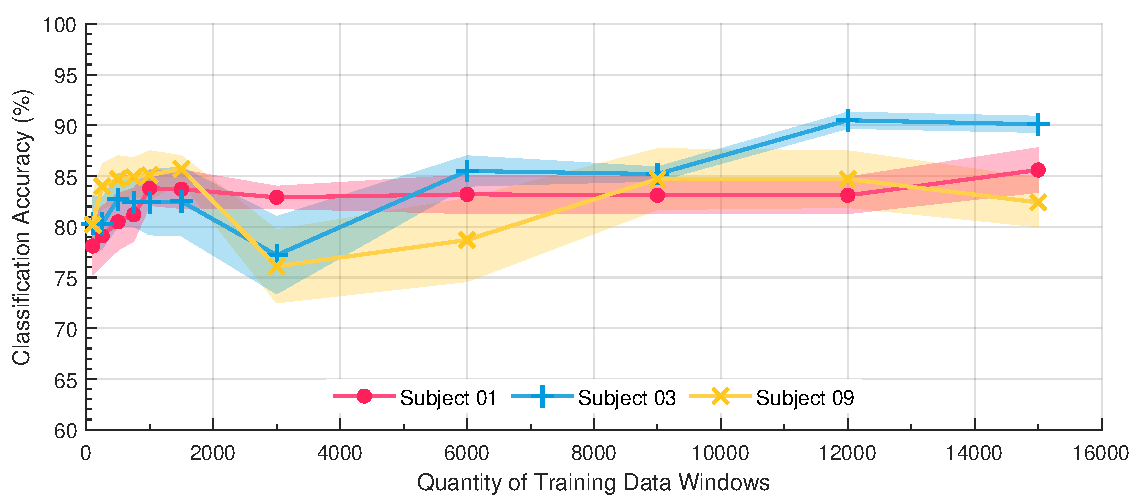
\includegraphics[width=\textwidth]{content/5-Personalisation/ch5_pre_trained_model_accuracy.pdf}
        \caption{Fine-tuning all layers}
        \label{subfig:ch5_fine-tuning-all-layers}
    \end{subfigure}
    \begin{subfigure}{\textwidth}
        \centering
        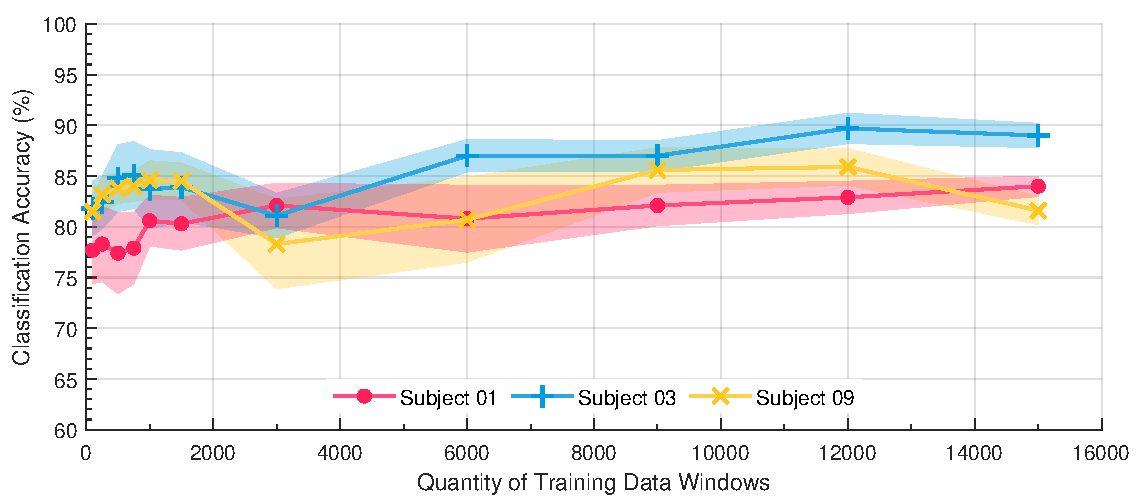
\includegraphics[width=\textwidth]{content/5-Personalisation/ch5_frozen_lstm_layer_accuracy.pdf}
        \caption{Fine-tuning only the dense layer}
    \end{subfigure}
    \caption[Results of fine-tuning a generic 32 unit \glsentryshort{lstm} model using increasing amounts of target data]{Results of fine-tuning a generic 32 unit \acrshort{lstm} model using increasing amounts of target data. The solid line represents the mean classification performance for each amount of training windows. The filled area represents the standard deviation $(n=25)$. Each of the 3 target subjects is represented individually. The red dot line is Subject 1, blue plus is subject 3 and yellow cross is subject 9.}
    \label{fig:ch5_pretrained_model}
\end{figure}
\begin{figure}[t]\ContinuedFloat
    \begin{subfigure}{\textwidth}
        \centering
        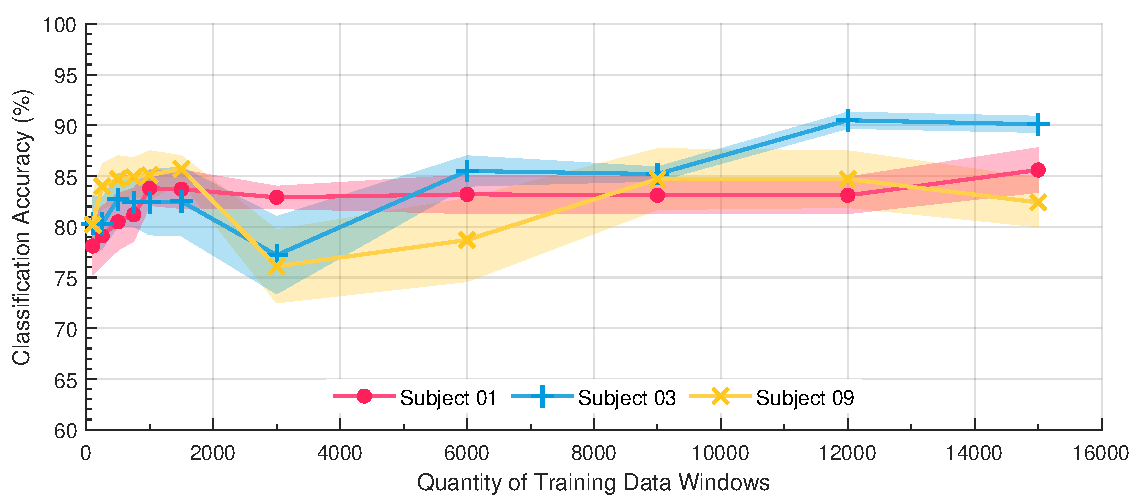
\includegraphics[width=\textwidth]{content/5-Personalisation/ch5_frozen_dense_layer_accuracy.pdf}
        \caption{Fine-tuning only the \acrshort{lstm} layer}
    \end{subfigure}
    \caption[]{Results of fine-tuning a generic 32 unit \acrshort{lstm} model using increasing amounts of target data (Cont.).}
\end{figure}

Figure \ref{subfig:ch5_fine-tuning-all-layers} shows the classification performance for fine-tuning all layers. The highest classification accuracy observed for each subject was $85.6\%$, $90.5\%$ and $84.7\%$ for subjects 1, 3 and 9 respectively. These were results were all achieved with either 12000 or 15000 target training windows. All models completed training in a small number of epochs, on average 5 with a 95\textsuperscript{th} percentile of 8.

Classification performance improves rapidly up to 1500 target training windows. When performance for 100, 250 and 500 training windows is compared to the bespoke baseline model performance is over 10\% better for all subjects. This potentially means only 30 seconds of each class are required. Performance improvements then increase more slowly with additional target data. The improvement over the bespoke model baseline also narrows to only a couple of percent.

Target windows quantities of 100-200 for subject 3 are also below the baseline performance. For subjects 3 and 9 performance drops down around 3000 target samples.  Other than these values all models exceed the baseline performance.

The drop in performance for higher values of training windows is still an improvement over the baselines for Subject 9 however briefly drops below the baseline general model for Subject 3. It's not obvious why this decrease in performance occurs but could be due to the introduction of a significantly different previously unseen environment to the training set.

Fine-tuning only the dense layer improved performance of Subject 3, no improvement for 9 and reduction in performance for 1. Standard deviation in general increased for all three subjects showing greater variation in performance across all models. When the dense layer was frozen there was a small improvement for subject 1 of greater than $1\%$ across all target window quantities but no meaningful change for subjects 3, and 9. Standard deviation remained largely the same when compared to fine-tuning all layers.

This approach to personalisation appears to give significant improvements in performance using only a small amount of target data. Only fine-tuning some layers doesn't give any consistent or meaningful improvement in performance.

%-------------------------------------------------------------------------------
\section{Discussion}
\label{sec:personalisation-discussion}
%What were we trying to achieve and have we achieved it?
The aim of this chapter was to develop methods that improve the performance of an \acrshort{lmr} network for a specific previously unseen individual. Improvements were measured in both computation efficiency and classification accuracy.

% Recap experiments
First a real world representative test scheme was developed. This presented the trained model with episode of activity that it had not previously seen. It gave a challenging data set as test performance was significantly below training performance. Given that the actual activity environment for each episode is not known it is difficult to asses how realistic this testing scheme is. 

Compared to the previous chapters work the data division scheme employed also reduced the amount of transition data that the model encountered. Data is cleaned it up. Previous work indicated these were a large source in inaccuracy which has not been considered in this work.

This was followed by establishing a baseline performance. The two baselines selected were performance of the novel test subject from a set of general models and performance of a model trained with only the target subjects data. These established a minimum performance that must be achieved for the personalisation techniques to be of merit.

%Do any of the methods show promise? Which model performed best
Both personalisation methods tested produced an improvement in accuracy which, depending on the quantity of target data, varied from greater than $10\%$ to just over a $2\%$ improvement over the baseline. So both were successful in achieving greater performance through personalisation. Both methods also reduced the quantity of target data required for the same classification when compared to the bespoke target models. However the data supplementation method required a significantly greater number of epochs than transfer learning to achieve this performance. For data supplementation it was also difficult to predict how much source data was needed so would implement in practice would be difficult. These results suggest that transfer learning is a better approach than data supplementation.

% How much data is required - results indicate you can never have enough. All models continued to improve with more data. Baseline, Supplementation and data grouping. All trained models gave the fastest early on, but although rate of improvement slowed down with increasing data it was still increasing.
All experiments investigated how much target data is required to achieve good performance. The results demonstrated that more data is better as should be expected. A plateauing of performance with increasing data was not seen implying additional data would likely have continued to improved performance. Performance improved most rapidly early therefore these method offer the best cost benefit at lower data quantities.

Collecting additional target data beyond what was collected rapidly becomes unrealistic. It is not possible to expose the model to every possible environment before deployment. A form of continuous on-line learning may well resolve this issue as well as allowing adaption to changes in individual gait characteristics over time.

% Data grouping might be improved by being more selective over which subjects are included. Literature supports this. Area for further work
For lower quantities of target data, data supplementation achieved better results than transfer learning. However due to the difficulties in predicting how much source data is required this a difficult system to implement. The in-precision of this technique is potentially at issue for this. More precision in the selection of which supplemental source data to use as shown in literature has the ability to improve performance. However additional measures would be needed to evaluate similarity between subjects, which are not needed when using purely deep learning approach. An alternative approach could be to bias learning towards the targets data as shown by Ferrari et al\cite{Ferrari2020}.

% Negative transfer with addition target windows - why might that be. Introduction of new previously unseen environments. Because the data set of the target subjects was so large its likely that the subjects visited the same environments/areas multiple times.
Transfer learning performance was more consistent in it's improvement in performance, performing better than baseline for the vast majority of tested configuration, apart from a few of test configurations. The anomalous results appear to come from the training sets used as they were repeated throughout all experiments. This may well be due to the introduction of new environments that present different gait characteristics from those previous seen in the data set. Due to the black box nature of each data recording it's not possible to know which kind of environment each episode is taken from. Therefore experimentation to determine if this hypothesis is true is not possible without collecting additional data with greater ground truth or controls.

% Freezing layers
The freezing of layers in the transfer learning did not result in any significant reduction in classification accuracy. For a model as small as was tested neither did it result in any significant improvement in computational performance. For more complex architectures however this could be a valuable technique for reducing computational training requirements as demonstrated by Yoon et al\cite{Yoon2017}.

Additional areas of research that could improve performance include the investigation of combined data supplementation and transfer learning methods; Additional investigation of model hyper-parameter and different model architectures.

The methods developed in this study will now be taken forward and applied to amputee data to determine if they are still applicable to subjects with abnormal gaits.

%-------------------------------------------------------------------------------
\section{Conclusions}
\label{sec:personalisation-conclusions}
The work in this chapter aimed to develop methods for personalisation of a \acrshort{lstm} \acrshort{lmr} network using a large source data set to supplement target data. These method will then be taken forward and applied to amputee data to try and reduce the data requirements.

Two methods were demonstrated, supplementing a target data to form an enlarged training set and fine-tuning a pre-trained general model. Both method were successful using the source data set to improve classification accuracy for the target users over the baseline. However the transfer learning approach achieved this performance in significantly fewer epochs requiring less computation resource.

After personalisation test subject 3 achieved a maximum classification accuracy of $90.5\%$ was achieved an improvement over $26.6\%$ over the baseline general model. The over two test subjects both achieved improvements of greater than $8.5\%$. When only a small amount of target training data is available, less than 30 seconds per activity class, performance of transfer learning is over 10\% better than training a model using only the target's data.

Following this study the methods developed will be tested using amputee data to see if these techniques can reduce the training data requirements for developing a classifier to improve the performance of a prosthetic limb.